
\makeatletter
\@ifundefined{standalonetrue}{\newif\ifstandalone}{}
\@ifundefined{section}{\standalonetrue}{\standalonefalse}
\makeatother
\ifstandalone
\documentclass{report}

\usepackage{textcase}
%\usepackage{hyperref}
%\hypersetup{breaklinks=true}


% Added packages
\usepackage[usenames]{color}
\usepackage{amsfonts, amsmath, amssymb, graphics}

% NOTE: bibentry MUST appear before the hyperref or build will fail
\usepackage{bibentry}
\nobibliography*
\usepackage[square,sort,comma,numbers]{natbib}
  
\usepackage{float}
\usepackage[
	hidelinks,%
    %hyperindex=true,		% Make numbers of index links as well
   	backref=page, 		% Provide page listing where refs occur in the bibliography
	%breaklinks=true,
    %colorlinks,%
    %citecolor=green,%
    %filecolor=blue,%
    %linkcolor=red,%
    %urlcolor=red, 
]{hyperref}

\usepackage{dsfont}
%%%% USEPACKAGES for MACROS %%%%%
\usepackage{algpseudocode}
\usepackage[chapter]{algorithm}
%\usepackage{caption}
\usepackage{subcaption}
\usepackage{url}

\usepackage{array}
\usepackage{arydshln}
\usepackage{multirow}
\usepackage{multicol}
%\usepackage[section]{placeins}

\usepackage[usenames,dvipsnames]{color}
%\usepackage[english]{babel}
\usepackage{tabularx}
\usepackage{soul}
\usepackage{xparse}
\usepackage{listings}
%\usepackage[normalem]{ulem}



%%%%%%%%%%%%%%%
% Show a list of items "todo" or "done" 
% USAGE: 
% \begin{todolist} 
% 	\todo Something not finished
% 	\done Something finished
% \end{todolist} 
\newenvironment{todolist}{%
  \begin{list}{}{}% whatever you want the list to be
  \let\olditem\item
  \renewcommand\item{\olditem \textcolor{red}{(TODO)}: }
  \newcommand\todo{\olditem \textcolor{red}{(TODO)}: }
   \newcommand\done{\olditem \textcolor{ForestGreen}{(DONE)}: }
}{%
  \end{list}
} 
%%%%%%%%%%%%%%%

%%%%%%%%%%%%%%%
% Show a Author's Note
% USAGE: 
% \incomplete[Optional footnote message to further clarify note]{The text which is currently not finished}
\DeclareDocumentCommand \incomplete{ o m }
{%
\IfNoValueTF {#1}
{\textcolor{red}{Incomplete: \ul{#2}}} 
{\textcolor{red}{Incomplete: \ul{#2}}\footnote{Comment: #1}}%
}
%%%%%%%%%%%%%%%



%%%%%%%%%%%%%%%
% Show a Author's Note
% USAGE: 
% \authnote[Optional footnote message to further clarify note]{The note to your readers}
\DeclareDocumentCommand \authnote { o m }
{%
\IfNoValueTF {#1}
{\textcolor{blue}{Author's Note: \ul{#2}}} 
{\textcolor{blue}{Author's Note: \ul{#2}}\footnote{Comment: #1}}%
}
%%%%%%%%%%%%%%%



%%%%%%%%%%%%%%%
% Strike out text that doesn't belong in the paper
% USAGE: 
% \strike[Optional footnote to state why it doesn't belong]{Text to strike out}
\DeclareDocumentCommand \strike { o m }
{%
\setstcolor{Red}
\IfNoValueTF {#1}
{\textcolor{Gray}{\st{#2}}} 
{\textcolor{Gray}{\st{#2}}\footnote{Comment: #1}}%
}
%%%%%%%%%%%%%%%

\definecolor{light-gray}{gray}{0.95}

\newcommand{\cbox}[3]{
\ \\
\fcolorbox{#1}{#2}{
\parbox{\textwidth}{
#3
}
}
}

% Setup an environment similar to verbatim but which will highlight any bash commands we have
\lstnewenvironment{unixcmds}[0]
{
%\lstset{language=bash,frame=shadowbox,rulesepcolor=\color{blue}}
\lstset{ %
language=sh,		% Language
basicstyle=\ttfamily,
backgroundcolor=\color{light-gray}, 
rulecolor=\color{blue},
%frame=tb, 
columns=fullflexible,
%framexrightmargin=-.2\textwidth,
linewidth=0.8\textwidth,
breaklines=true,
%prebreak=/, 
  prebreak = \raisebox{0ex}[0ex][0ex]{\ensuremath{\hookleftarrow}},
%basicstyle=\footnotesize,       % the size of the fonts that are used for the code
%numbers=left,                   % where to put the line-numbers
%numberstyle=\footnotesize,      % the size of the fonts that are used for the line-numbers
%stepnumber=2,                   % the step between two line-numbers. If it's 1 each line 
                                % will be numbered
%numbersep=5pt,                  % how far the line-numbers are from the code
showspaces=false,               % show spaces adding particular underscores
showstringspaces=false,         % underline spaces within strings
showtabs=false,                 % show tabs within strings adding particular underscores
frame=single,	                % adds a frame around the code
tabsize=2,	                % sets default tabsize to 2 spaces
captionpos=b,                   % sets the caption-position to bottom
breakatwhitespace=false,        % sets if automatic breaks should only happen at whitespace
}
} { }

% Setup an environment similar to verbatim but which will highlight any bash commands we have
\lstnewenvironment{cppcode}[1]
{
%\lstset{language=bash,frame=shadowbox,rulesepcolor=\color{blue}}
\lstset{ %
	backgroundcolor=\color{light-gray}, 
	rulecolor=\color[rgb]{0.133,0.545,0.133},
	tabsize=4,
	language=[GNU]C++,
%	basicstyle=\ttfamily,
        basicstyle=\scriptsize,
        upquote=true,
        aboveskip={1.5\baselineskip},
        columns=fullflexible,
        %framexrightmargin=-.1\textwidth,
       %framexleftmargin=6mm,
        showstringspaces=false,
        extendedchars=true,
        breaklines=true,
        prebreak = \raisebox{0ex}[0ex][0ex]{\ensuremath{\hookleftarrow}},
        frame=single,
        showtabs=false,
        showspaces=false,
        showstringspaces=false,
        numbers=left,                   % where to put the line-numbers
	numberstyle=\footnotesize,      % the size of the fonts that are used for the line-numbers
	stepnumber=4,                   % the step between two line-numbers. If it's 1 each line 
                                % will be numbered
	firstnumber=#1,
         numbersep=5pt,                  % how far the line-numbers are from the code
        identifierstyle=\ttfamily,
        keywordstyle=\color[rgb]{0,0,1},
        commentstyle=\color[rgb]{0.133,0.545,0.133},
        stringstyle=\color[rgb]{0.627,0.126,0.941},
}
} { }

% Setup an environment similar to verbatim but which will highlight any bash commands we have
\lstnewenvironment{mcode}[1]
{
\lstset{ %
	backgroundcolor=\color{light-gray}, 
	rulecolor=\color[rgb]{0.133,0.545,0.133},
	tabsize=4,
	language=Matlab,
%	basicstyle=\ttfamily,
        basicstyle=\scriptsize,
        upquote=true,
        aboveskip={1.5\baselineskip},
        columns=fullflexible,
        %framexrightmargin=-.1\textwidth,
       %framexleftmargin=6mm,
        showstringspaces=false,
        extendedchars=true,
        breaklines=true,
        prebreak = \raisebox{0ex}[0ex][0ex]{\ensuremath{\hookleftarrow}},
        frame=single,
        showtabs=false,
        showspaces=false,
        showstringspaces=false,
        numbers=left,                   % where to put the line-numbers
	numberstyle=\footnotesize,      % the size of the fonts that are used for the line-numbers
	stepnumber=4,                   % the step between two line-numbers. If it's 1 each line 
                                % will be numbered
	firstnumber=#1,
         numbersep=5pt,                  % how far the line-numbers are from the code
        identifierstyle=\ttfamily,
        keywordstyle=\color[rgb]{0,0,1},
        commentstyle=\color[rgb]{0.133,0.545,0.133},
        stringstyle=\color[rgb]{0.627,0.126,0.941},
}
} { }

\newcommand{\inputmcode}[1]{%
\lstset{ %
	backgroundcolor=\color{light-gray},  %
	rulecolor=\color[rgb]{0.133,0.545,0.133}, %
	tabsize=4, %
	language=Matlab, %
%	basicstyle=\ttfamily,
        basicstyle=\scriptsize, %
        %        upquote=true,
        aboveskip={1.5\baselineskip}, %
        columns=fullflexible, %
        %framexrightmargin=-.1\textwidth,
       %framexleftmargin=6mm,
        showstringspaces=false, %
        extendedchars=true, %
        breaklines=true, %
        prebreak = \raisebox{0ex}[0ex][0ex]{\ensuremath{\hookleftarrow}}, %
        frame=single, %
        showtabs=false, %
        showspaces=false, %
        showstringspaces=false,%
        numbers=left,                   % where to put the line-numbers
	numberstyle=\footnotesize,      % the size of the fonts that are used for the line-numbers
	stepnumber=4,                   % the step between two line-numbers. If it's 1 each line 
                                % will be numbered
         numbersep=5pt,                  % how far the line-numbers are from the code
        identifierstyle=\ttfamily, %
        keywordstyle=\color[rgb]{0,0,1}, %
        commentstyle=\color[rgb]{0.133,0.545,0.133}, %
        stringstyle=\color[rgb]{0.627,0.126,0.941} %
}
\lstinputlisting{#1}%
}

%\lstset{ %
%	backgroundcolor=\color{light-gray}, 
%	rulecolor=\color[rgb]{0.133,0.545,0.133},
%	tabsize=4,
%	language=Matlab,
%%	basicstyle=\ttfamily,
%        basicstyle=\scriptsize,
%        upquote=true,
%        aboveskip={1.5\baselineskip},
%        columns=fullflexible,
%        %framexrightmargin=-.1\textwidth,
%       %framexleftmargin=6mm,
%        showstringspaces=false,
%        extendedchars=true,
%        breaklines=true,
%        prebreak = \raisebox{0ex}[0ex][0ex]{\ensuremath{\hookleftarrow}},
%        frame=single,
%        showtabs=false,
%        showspaces=false,
%        showstringspaces=false,
%        numbers=left,                   % where to put the line-numbers
%	numberstyle=\footnotesize,      % the size of the fonts that are used for the line-numbers
%	stepnumber=4,                   % the step between two line-numbers. If it's 1 each line 
%                                % will be numbered
%	firstnumber=#1,
%         numbersep=5pt,                  % how far the line-numbers are from the code
%        identifierstyle=\ttfamily,
%        keywordstyle=\color[rgb]{0,0,1},
%        commentstyle=\color[rgb]{0.133,0.545,0.133},
%        stringstyle=\color[rgb]{0.627,0.126,0.941},
%}


\newcommand{\Laplacian}[1]{\nabla^2 #1}

% set of all nodes received and contained on GPU
\newcommand{\setAllNodes}[0]{\mathcal{G}}
% set of stencil centers on GPU
\newcommand{\setCenters}[0]{\mathcal{Q}}
% set of stencil centers with nodes in \setDepend
\newcommand{\setBoundary}[0]{\mathcal{B}}
% set of nodes received by other GPUs
\newcommand{\setDepend}[0]{\mathcal{R}}
% set of nodes sent to other GPUs
\newcommand{\setProvide}[0]{\mathcal{O}}


\newcommand{\toprule}[0]{\hline}
\newcommand{\midrule}[0]{\hline\hline}
\newcommand{\bottomrule}[0]{\hline}

\newcolumntype{C}{>{\centering\arraybackslash}b{1in}}
\newcolumntype{L}{>{\flushleft\arraybackslash}b{1.5in}}
\newcolumntype{R}{>{\flushright\arraybackslash}b{1.5in}}
\newcolumntype{D}{>{\flushright\arraybackslash}b{2.0in}}
\newcolumntype{E}{>{\flushright\arraybackslash}b{1.0in}}

\DeclareSymbolFont{AMSb}{U}{msb}{m}{n}
\DeclareMathSymbol{\N}{\mathbin}{AMSb}{"4E}
\DeclareMathSymbol{\Z}{\mathbin}{AMSb}{"5A}
\DeclareMathSymbol{\R}{\mathbin}{AMSb}{"52}
\DeclareMathSymbol{\Q}{\mathbin}{AMSb}{"51}
\DeclareMathSymbol{\PP}{\mathbin}{AMSb}{"50}
\DeclareMathSymbol{\I}{\mathbin}{AMSb}{"49}
%\DeclareMathSymbol{\C}{\mathbin}{AMSb}{"43}

%%%%%% VECTOR NORM: %%%%%%%
\newcommand{\vectornorm}[1]{\left|\left|#1\right|\right|}
\newcommand{\vnorm}[1]{\left|\left|#1\right|\right|}
\newcommand{\by}[0]{\times}
\newcommand{\vect}[1]{\mathbf{#1}}
%\newcommand{\mat}[1]{\mathbf{#1}} 

%\renewcommand{\vec}[1]{ \textbf{#1} }
%%%%%%%%%%%%%%%%%%%%%%

%%%%%%% THM, COR, DEF %%%%%%%
%\newtheorem{theorem}{Theorem}[section]
%\newtheorem{lemma}[theorem]{Lemma}
%\newtheorem{proposition}[theorem]{Proposition}
%\newtheorem{corollary}[theorem]{Corollary}
%\newenvironment{proof}[1][Proof]{\begin{trivlist}
%\item[\hskip \labelsep {\bfseries #1}]}{\end{trivlist}}
%\newenvironment{definition}[1][Definition]{\begin{trivlist}
%\item[\hskip \labelsep {\bfseries #1}]}{\end{trivlist}}
%\newenvironment{example}[1][Example]{\begin{trivlist}
%\item[\hskip \labelsep {\bfseries #1}]}{\end{trivlist}}
%\newenvironment{remark}[1][Remark]{\begin{trivlist}
%\item[\hskip \labelsep {\bfseries #1}]}{\end{trivlist}}
%\newcommand{\qed}{\nobreak \ifvmode \relax \else
%      \ifdim\lastskip<1.5em \hskip-\lastskip
%      \hskip1.5em plus0em minus0.5em \fi \nobreak
%      \vrule height0.75em width0.5em depth0.25em\fi}
%%%%%%%%%%%%%%%%%%%%%%

%
%\usepackage[algochapter]{algorithm2e}
%\usepackage[usenames]{color}
% colors to show the corrections
\newcommand{\red}[1]{\textbf{\textcolor{red}{#1}}}
\newcommand{\blue}[1]{\textbf{\textcolor{blue}{#1}}}
\newcommand{\cyan}[1]{\textbf{\textcolor{cyan}{#1}}}
\newcommand{\green}[1]{\textbf{\textcolor{green}{#1}}}
\newcommand{\magenta}[1]{\textbf{\textcolor{magenta}{#1}}}
\newcommand{\orange}[1]{\textbf{\textcolor{orange}{#1}}}
%%%%%%%%%% DK DK
% comments between authors
\newcommand{\toall}[1]{\textbf{\green{@@@ All: #1 @@@}}}
\newcommand{\toevan}[1]{\textbf{\red{*** Evan: #1 ***}}}
%\newcommand{\toevan}[1]{}  % USE FOR FINAL VERSION
\newcommand{\toe}[1]{\textbf{\red{*** Evan: #1 ***}}}
\newcommand{\tog}[1]{\textbf{\blue{*** Gordon: #1 ***}}}
%\newcommand{\togordon}[1]{\textbf{\blue{*** Gordon: #1 ***}}}
\renewcommand{\ge}[3]{{\textcolor{blue}{*** \textbf{Gordon:}\strike{#1} #2 ***}}\red{(#3)}}
\renewcommand{\ge}[3]{{\textcolor{blue}{#2}}}
\renewcommand{\ge}[3]{{\textcolor{Red}{#2}}}
\newcommand{\eb}[3]{{\textcolor{Red}{*** \textbf{Evan:}\strike{#1} #2 ***}}\red{(#3)}}
\renewcommand{\eb}[3]{{{\textcolor{Red}{#2}}}}
%\def\ge#1#2#3{}{\textbf{\blue{*** Gordon: #2 ***}}}{(#3)}
\newcommand{\gee}[1]{{\bf{\blue{{\em #1}}}}}
\newcommand{\old}[1]{}
\newcommand{\del}[1]{***#1*** }



% \DeclareMathOperator{\Sample}{Sample}
%\let\vaccent=\v % rename builtin command \v{} to \vaccent{}
%\renewcommand{\vec}[1]{\ensuremath{\mathbf{#1}}} % for vectors
\newcommand{\gv}[1]{\ensuremath{\mbox{\boldmath$ #1 $}}} 
% for vectors of Greek letters
\newcommand{\uv}[1]{\ensuremath{\mathbf{\hat{#1}}}} % for unit vector
\newcommand{\abs}[1]{\left| #1 \right|} % for absolute value
\newcommand{\avg}[1]{\left< #1 \right>} % for average
\let\underdot=\d % rename builtin command \d{} to \underdot{}
\renewcommand{\d}[2]{\frac{d #1}{d #2}} % for derivatives
\newcommand{\dd}[2]{\frac{d^2 #1}{d #2^2}} % for double derivatives
\newcommand{\pd}[2]{\frac{\partial #1}{\partial #2}} 
% for partial derivatives
\newcommand{\pdd}[2]{\frac{\partial^2 #1}{\partial #2^2}} 
\newcommand{\pdda}[3]{\frac{\partial^2 #1}{\partial #2 \partial #3}} 
% for double partial derivatives
\newcommand{\pdc}[3]{\left( \frac{\partial #1}{\partial #2}
 \right)_{#3}} % for thermodynamic partial derivatives
\newcommand{\ket}[1]{\left| #1 \right>} % for Dirac bras
\newcommand{\bra}[1]{\left< #1 \right|} % for Dirac kets
\newcommand{\braket}[2]{\left< #1 \vphantom{#2} \right|
 \left. #2 \vphantom{#1} \right>} % for Dirac brackets
\newcommand{\matrixel}[3]{\left< #1 \vphantom{#2#3} \right|
 #2 \left| #3 \vphantom{#1#2} \right>} % for Dirac matrix elements
\newcommand{\grad}[1]{\gv{\nabla} #1} % for gradient
\let\divsymb=\div % rename builtin command \div to \divsymb
\renewcommand{\div}[1]{\gv{\nabla} \cdot #1} % for divergence
\newcommand{\curl}[1]{\gv{\nabla} \times #1} % for curl
\let\baraccent=\= % rename builtin command \= to \baraccent
\renewcommand{\=}[1]{\stackrel{#1}{=}} % for putting numbers above =
\newcommand{\diffop}[1]{\mathcal{L}#1}
\newcommand{\boundop}[1]{\mathcal{B}#1}
\newcommand{\rvec}[0]{{\bf r}}

\newcommand{\Interior}[0]{\Omega}
\newcommand{\domain}[0]{\Omega}
%\newcommand{\Boundary}[0]{\partial \Omega}
\newcommand{\Boundary}[0]{\Gamma}

\newcommand{\on}[1]{\hskip1.5em \textrm{ on } #1}

\newcommand{\gemm}{\texttt{GEMM}}
\newcommand{\trmm}{\texttt{TRMM}}
\newcommand{\gesvd}{\texttt{GESVD}}
\newcommand{\geqrf}{\texttt{GEQRF}}


\newcommand{\minitab}[2][l]{\begin{tabular}{#1}#2\end{tabular}}
\newcommand{\comm}[1]{\textcolor{red}{\textit{#1}}}

\newcommand{\nfrac}[2]{
\nicefrac{#1}{#2}
%\frac{#1}{#2}
}

\usepackage{xparse}
\usepackage{soul}


%%%%%%%%%%%%%%%
% Show a Author's Note
% USAGE: 
% \incomplete[Optional footnote message to further clarify note]{The text which is currently not finished}
\DeclareDocumentCommand \incomplete{ o m }
{%
\IfNoValueTF {#1}
{\textcolor{red}{Incomplete: \ul{#2}}} 
{\textcolor{red}{Incomplete: \ul{#2}}\footnote{Comment: #1}}%
}
%%%%%%%%%%%%%%%



%%%%%%%%%%%%%%%
% Show a Author's Note
% USAGE: 
% \authnote[Optional footnote message to further clarify note]{The note to your readers}
\DeclareDocumentCommand \authnote { o m }
{%
\IfNoValueTF {#1}
{\textcolor{blue}{Author's Note: \ul{#2}}} 
{\textcolor{blue}{Author's Note: \ul{#2}}\footnote{Comment: #1}}%
}
%%%%%%%%%%%%%%%



%%%%%%%%%%%%%%%
% Strike out text that doesn't belong in the paper
% USAGE: 
% \strike[Optional footnote to state why it doesn't belong]{Text to strike out}
\DeclareDocumentCommand \strike { o m }
{%
\setstcolor{red}
\IfNoValueTF {#1}
{\textcolor{Gray}{\st{#2}}} 
{\textcolor{Gray}{\st{#2}}\footnote{Comment: #1}}%
}
%%%%%%%%%%%%%%%



%
% colors to show the corrections
\newcommand{\red}[1]{\textbf{\textcolor{red}{#1}}}
\newcommand{\blue}[1]{\textbf{\textcolor{blue}{#1}}}
\newcommand{\cyan}[1]{\textbf{\textcolor{cyan}{#1}}}
\newcommand{\green}[1]{\textbf{\textcolor{green}{#1}}}
\newcommand{\magenta}[1]{\textbf{\textcolor{magenta}{#1}}}
\newcommand{\orange}[1]{\textbf{\textcolor{orange}{#1}}}
%%%%%%%%%% DK DK
% comments between authors
\newcommand{\toall}[1]{\textbf{\green{@@@ All: #1 @@@}}}
\newcommand{\toevan}[1]{\textbf{\red{*** Evan: #1 ***}}}
%\newcommand{\toevan}[1]{}  % USE FOR FINAL VERSION
\newcommand{\toe}[1]{\textbf{\red{*** Evan: #1 ***}}}
\newcommand{\tog}[1]{\textbf{\blue{*** Gordon: #1 ***}}}
%\newcommand{\togordon}[1]{\textbf{\blue{*** Gordon: #1 ***}}}
\renewcommand{\ge}[3]{{\textcolor{blue}{*** \textbf{Gordon:}\strike{#1} #2 ***}}\red{(#3)}}
\renewcommand{\ge}[3]{{\textcolor{blue}{#2}}}
\renewcommand{\ge}[3]{{\textcolor{red}{#2}}}
\newcommand{\eb}[3]{{\textcolor{red}{*** \textbf{Evan:}\strike{#1} #2 ***}}\red{(#3)}}
\renewcommand{\eb}[3]{{{\textcolor{red}{#2}}}}
%\def\ge#1#2#3{}{\textbf{\blue{*** Gordon: #2 ***}}}{(#3)}
\newcommand{\gee}[1]{{\bf{\blue{{\em #1}}}}}
\newcommand{\old}[1]{}
\newcommand{\del}[1]{***#1*** }



% Rename  this file          misc_mac.tex
%----------------------------------------------------------------------
%%%%%%%%%%%%%%%%%%%%%%%%%%%%%%%%%%%%%%%%%%%%%%%%%%%%%%%%%%%%%%%%%%%%%%%%%%%%%%%
%
%	Math Symbols   Math Symbols   Math Symbols   Math Symbols   
%
%%%%%%%%%%%%%%%%%%%%%%%%%%%%%%%%%%%%%%%%%%%%%%%%%%%%%%%%%%%%%%%%%%%%%%%%%%%%%%%
\def\pmb#1{\setbox0=\hbox{$#1$}%
	\kern-.025em\copy0\kern-\wd0
	\kern.05em\copy0\kern-\wd0
	\kern-.025em\raise.0433em\box0}
\def\pmbf#1{\pmb#1}
\def\bfg#1{\pmb#1}

% BETTER VALUES FOR AUTOMATIC FIGURE PLACEMENT THAN THOSE PROVIDED BY 
% LATEX DEFAULTS.

\renewcommand{\textfloatsep}{1ex}
\renewcommand{\floatpagefraction}{0.9}
\renewcommand{\intextsep}{1ex}
\renewcommand{\topfraction}{.9}
\renewcommand{\bottomfraction}{.9}
\renewcommand{\textfraction}{.1}

% #1  position of floating figure (h|t|b|p)
% #1  EPS postscript file
% #2  size
% #3  caption

%usage of newfig:
%  \newfig{file.ps}{3in}{Fig1: this is a figure}

\input{epsf}
\def\newfig#1#2#3{
  \begin{figure}[htbp]
  \vspace{1ex}
  \setlength{\epsfxsize}{#2}
  \centerline{\epsfbox{#1}}
  \vspace{-.1in}\caption{\small #3}\break\vspace{.2in}
  \label{#1}
  \end{figure}
}

%usage of newfigtwo: 2 figures, vertically stacked
% \newfig
%	{file1.ps}
%	{file2.ps}
%	{width}
%	{vertical space}
%	{Caption}

\def\newfigtwo#1#2#3#4#5{
  \begin{figure}[htbp]
  \vspace{1ex}
  \setlength{\epsfxsize}{#3}
  \centerline{\epsfbox{#1}}
  \vspace{#4}
  \setlength{\epsfxsize}{#3}
  \centerline{\epsfbox{#2}}
  \vspace{-.1in}\caption{\small #5}\break\vspace{.2in}
  \label{#1}
  \end{figure}
}

\def\newfigh#1#2#3#4{  % add height specification
  \begin{figure}[htbp]
  \vspace{1ex}
  \setlength{\epsfxsize}{#2}
  \setlength{\epsfysize}{#4}
  \centerline{\epsfbox{#1}}
  \vspace{-.1in}\caption{\small #3}\break\vspace{.2in}
  \label{#1}
  \end{figure}
}

\def\herefig#1#2#3{
  \begin{figure}[h]
  \setlength{\epsfxsize}{#2}
  \centerline{\epsfbox{#1}}
  \caption{\small #3}
  \label{#1}
  \end{figure}
}

\def\etal{{{\em et~al.\,\,}}}
\def\note#1{\\ =====#1===== \\}
\def\FBOX#1{\ \\ \fbox{\begin{minipage}{5in}#1\end{minipage}}\\ }
\newcount\sectionno     \sectionno=0
\newcount\eqnum         \eqnum=0
\def\addeqno{\global\advance \eqnum by  1 }
\def\subeqno{\global\advance \eqnum by -1 }
%\def\eqn{\addeqno \eqno \hbox{(\number\sectionno.\number\eqnum)} }

\def\tildetilde#1{\tilde{\tilde{#1}}}
\def\barbar#1{\overbar{\overbar{#1}}}

\def\vsp#1{\vspace{#1 ex}}
\def\fpar{\hspace{\parindent}}
%
%  \pf : 2 arguments: numerator and denominator of partial derivative
%
\def\pf#1#2{{\frac{\partial{#1}}{\partial{#2}}}}
\def\pfs#1#2{{\partial_{#2}{#1}}}
\def\pftwo#1#2{{\frac{\partial^2{#1}}{\partial{#2}^2}}}
\def\pfxx#1#2{{\frac{\partial^2{#1}}{\partial{#2}^2}}}
%\def\pfxy#1#2{{\frac{\partial^2{#1}}{\partial{#2}\partial{#3}}}}
\def\pfn#1#2#3{{\frac{\partial^{#1}{#2}}{\partial{#3}^{#1}}}}
\def\df#1#2{{\frac{d{#1}}{d{#2}}}}
\def\dfn#1#2#3{{\frac{d^{#1}{#2}}{d{#3}^{#1}}}}
\def\Dt#1#2{\frac{D#1}{D#2}}
\def\dt#1#2{\frac{d#1}{d#2}}
\def\bld#1{{\bf #1}}
\def\pfp#1#2#3{\pf{}{#3}{\left(\frac{#1}{#2}\right)}}

\def\norm#1{\|#1\|}

%
% Graphic characters  (\dot already defined by TeX/LateX)
%
\def\dash{\rule[1.5pt]{2mm}{.3mm}\HS{.9mm}}
\def\dott{\rule[1.5pt]{.7mm}{.3mm}\HS{.7mm}}
\def\dashline{\dash\dash\dash}
\def\dotline{\dott\dott\dott\dott\dott\dott}
\def\dashdotline{\dash$\cdot$\HS{.9mm}\dash}
\def\solidline{\rule[2pt]{7mm}{.3mm}}
% 
% overcircle
%
\def\ovcircle#1{\buildrel{\circ}\over{#1}}
%\def\below#1#2{\buildrel{#2}\under{#1}}
%\def\above#1#2{\buildrel{#2}\over{#1}}
%
%  big parenthesis and brackets
%
\def\bigpar#1#2{{\left(\frac{#1}{#2}\right)}}
\def\bigbra#1#2{{\left\[\frac{#1}{#2}\right\]}}

\def\Lp{\left(}
\def\Rp{\right)}
\def\Lb{\left[}
\def\Rb{\right]}
\def\Ln{\left\langle}
\def\Rn{\right\rangle}
\def\Ld{\left.}
\def\Rd{\right.}
\def\Lv{\left|}
\def\Rv{\right|}
\def\Lbr{\left|}
\def\Rbr{\right|}
\def\lng{\langle}
\def\rng{\rangle}
\def\Lc{\left\{}
\def\Rc{\right\}}
%%% %

% Cannot be handled by Lyx
%\def\[{{[}}
%\def\]{{]}}

%
\def\eol{\nonumber \\}
\def\eolnonb{\nonumber\\}
\def\eolnb{\\}
\def\nonb{\nonumber}
\def\be{\begin{equation}}
\def\ee{\end{equation}}
\def\BEQNA{\begin{eqnarray}}
\def\EEQNA{\end{eqnarray}}
\def\eqa{&=&}
\def\beqna{\begin{eqnarray}}
\def\eeqna{\end{eqnarray}}
\def\bverb{\begin{verbatim}}
\def\everb{\end{verbatim}}
\def\VERB#1{\bverb #1 \everb}
\def\btbl{\begin{tabular}}
\def\etbl{\end{tabular}}
\def\bmini{\begin{minipage}[t]{5.5in}}
\def\emini{\end{minipage}}
\def\parray#1#2{\left(\begin{array}{#1}#2\end{array}\right)}
\def\barray#1#2{\left[\begin{array}{#1}#2\end{array}\right]}
\def\carray#1#2{\left\{\begin{array}{#1}#2\end{array}\right.}
\def\darray#1#2{\left|\begin{array}{#1}#2\end{array}\right|}

\def\BEGTABLE#1{\begin{table}[hbt]\vspace{2ex}\begin{center}\bmini\centering\btbl{#1}}
\def\ENDTABLE#1#2{\etbl\caption[#1]{#2}\EMINI\end{center}\vspace{2ex}\end{table}}

\def\bfltbl#1{\begin{table}[hbt]\vspace{2ex}\begin{center}\bmini\centering\btbl{#1}}
\def\efltbl#1#2{\etbl\caption[#1]{#2}\emini\end{center}\vspace{2ex}\end{table}}
\def\mcol{\multicolumn}
%
%  label equations with (#)
%
\def\reff#1{(\ref{#1})}
%
%  macros borrowed from viewgraph package
%

\newenvironment{LETTRS}[3]{\begin{letter}{#1}
\input{origin}\opening{Dear #2:}\input{#3}\closing{Sincerely yours,}\end{letter}}{\clearpage}

\newenvironment{VIEW}[1]{{\BC\Huge\bf #1 \EC}\LARGE\VS{.05in}}{\clearpage}

\def\RM#1{\rm{#1\ }}
\def\BV{\begin{VIEW}}
\def\EV{\end{VIEW}}

\def\NI{\noindent}

\def\VS{\vspace*}
\def\HS{\hspace*}
\def\IT{\item}

\def\BARR{\begin{array}}
\def\EARR{\end{array}}

\def\BPARR{\left(\begin{array}}
\def\EPARR{\end{array}\right)}

\def\BDET{\left|\begin{array}}
\def\EDET{\end{array}\right|}

\def\BDF{\begin{definition}}
\def\EDF{\end{definition}}

\def\BSU{\begin{block}{Summary}}
\def\ESU{\end{block}}

\def\BEX{\begin{example}}
\def\EEX{\end{example}}

\def\BTH{\begin{theorem}}
\def\ETH{\end{theorem}}

\def\BCO{\begin{corollary}}
\def\ECO{\end{corollary}}

\def\BPROOF{\begin{proof}}
\def\EPROOF{\end{proof}}

\def\BLM{\begin{lemma}}
\def\ELM{\end{lemma}}

\def\BEQ{\begin{equation}}
\def\EEQ{\end{equation}}

\def\BEQNNB{$$}
\def\EEQNNB{$$}

\def\BE{\begin{enumerate}}
\def\EE{\end{enumerate}}

\def\BD{\begin{description}}
\def\ED{\end{description}}

\def\BI{\begin{itemize}}
\def\EI{\end{itemize}}

\def\BC{\begin{center}}
\def\EC{\end{center}}

\def\BFIG{\begin{figure}}
\def\EFIG{\end{figure}}

\def\BTABB{\begin{tabbing}}
\def\ETABB{\end{tabbing}}

\def\BMINI{\begin{minipage}}
\def\EMINI{\end{minipage}}

\def\BTABLE{\begin{table}}
\def\ETABLE{\end{table}}

\def\BTABUL{\begin{tabular}}
\def\ETABUL{\end{tabular}}

\def\MCOL{\multicolumn}
\def\UL{\underline}
\def\ULL#1{\UL{\UL{#1}}}

\def\BDOC{\begin{document}}
\def\EDOC{\end{document}}

\def\EM#1{{\em #1\/}}
\def\FN{\footnote}

% Courtesy of Ugo Piomelli

\def\latexfig #1 #2 #3 #4 #5 {\ \vfill
\hfill\hbox to 0.05in{\vbox to #3truein{
         \special{psfile="#1" angle=270 hscale=100 
                  hoffset=#4 voffset=#5 vscale=100} }\hfill}
\hfill\vspace{-0.1in}        }

% #1 is the .ps filename
% #2 is not used in the present version
% #3 is the size of the white space left above the caption (in inches)
% #4 is the horizontal offset from some unknown reference point.
%    It is in 1/72 of an inch and is positive to the right.
% #5 is the vertical offset from some unknown reference point.
%    It is in 1/72 of an inch and is positive upwards.


\newcommand{\mathsym}[1]{{}}
\newcommand{\unicode}[1]{{}}
\newcommand{\ep}{\epsilon}
\newcommand{\vv}{\mathbf{v}}
\newcommand{\vu}{\mathbf{u}}
\newcommand{\vx}{\mathbf{x}}

\newcommand{\Laplacian}[1]{\nabla^2 #1}
\newcommand{\LaplaceBeltrami}[1]{\Delta_S #1}

% set of all nodes received and contained on GPU
\newcommand{\setAllNodes}[0]{\mathcal{G}}
% set of stencil centers on GPU
\newcommand{\setCenters}[0]{\mathcal{Q}}
% set of stencil centers with nodes in \setDepend
\newcommand{\setBoundary}[0]{\mathcal{B}}
% set of nodes received by other GPUs
\newcommand{\setDepend}[0]{\mathcal{R}}
% set of nodes sent to other GPUs
\newcommand{\setProvide}[0]{\mathcal{O}}





\usepackage{tabularx} 
\newcolumntype{C}{>{\centering\arraybackslash}b{1in}}
\newcolumntype{L}{>{\flushleft\arraybackslash}b{1.5in}}
\newcolumntype{R}{>{\flushright\arraybackslash}b{1.5in}}
\newcolumntype{D}{>{\flushright\arraybackslash}b{2.0in}}
\newcolumntype{E}{>{\flushright\arraybackslash}b{1.0in}}


 


%\usepackage{xcolor}

%\usepackage{refcheck}
% Sepia
%\definecolor{myBGcolor}{HTML}{F6F0D6}
%\definecolor{myTextcolor}{HTML}{4F452C}
% Dark
%\definecolor{myBGcolor}{HTML}{3E3535}
%\definecolor{myTextcolor}{HTML}{CFECEC}
%\color{myTextcolor}
%\pagecolor{myBGcolor}
 
\usepackage[margin=1.25in]{geometry}

\begin{document}
\fi


\chapter{Distributed RBF-FD (incomplete)}
\label{chap:distributed_rbffd}


%TODO: Similar Overlapping algorithm: \url{http://arxiv.org/pdf/1101.0091v1.pdf}
 %Imbalanced computation can be the source of excessive delays as processors sit idle and wait for other processors to catch up. 

Parallelizing applications in a distributed computing environment requires three
design decisions \cite{Saad2003}: 
\begin{enumerate} 
\item Partition the problem to distribute work across multiple processes. Intelligent partitioning
impacts load balancing and communication latency.
\item Determine the subset of node information,
solution values, etc. that are visible to each process, and establish index mappings that translate between a local context and the global problem. 
\item Establish a local ordering of data. The right local order can improve solver performance and/or simplify data movement. %Of particular interest here is how to minimize data movement at each iteration. In Chapter~\ref{chap:multigpu_rbffd} the local ordering will help minimize data transfer between CPU and GPU. 
\end{enumerate}

This chapter details the first implementation of RBF-FD designed for distributed computing environments and a few optimizations that help scale computation across a thousand processes. 

We operate under the assumption that inter-process communication is managed by the \emph{Message Passing Interface (MPI)} \cite{MPI}. Details on how communication collectives are used are included below in Section~\ref{sec:mpi_collectives}. 



\section{Partitioning}

We start with the concept of a \emph{domain}, which is partitioned into a set of \emph{sub-domains}. %TODO: elaborate



For ease of development and parallel debugging, partitioning is initially
assumed to be linear along the $x$-axis. This approach is not uncommon when solving PDEs on rectangular domains (see e.g., \cite{Divo2007, Thibault2009}). However, on irregular domains a simple one-dimensional cut can result in imbalanced workloads across processors. 

% A similar decomposition occurs in \cite{Divo2007} where the authors apply a local RBF collocation scheme to model viscous flow and heat transfer on rectangular domains. Thibault and Senocak  \cite{Thibault2009} partition a rectangular domain along the $z$-dimension for a variety of 3-D fluid benchmarks. 

Figure~\ref{fig:decomposed_sphere} illustrates a partitioning of
$N=10,201$ nodes on the unit sphere for four processes. 
Each partition, illustrated as a unique color, contains many stencil centers. 
Based on the location of a stencil's center the corresponding partition is easily identified. In cases where stencils are part of one partition and depend on stencil nodes in another, we say that the dependencies are \emph{ghost nodes}. %TODO: need ghost node ref.
In many cases, ghost nodes are treated the same as any other stencil node. The CPU process in charge of a partition is fully aware of the ghost node coordinate, current solution value(s), etc. However, values at ghost nodes are modified by another process, so changes must be explicitly synchronized via MPI in order to maintain consistency. 

In Figure~\ref{fig:decomposed_sphere}, alternating representations between node points and interpolated surfaces illustrates the
overlap regions where ghost nodes reside. Due to stencil dependencies in each partition, the overlap region representations are double-wide---i.e., they contain a set of ghost nodes for both the left and right partitions. 

As the stencil size increases, the width of the
overlap regions relative to total number of nodes on the sphere proportionally increases. In Figure~\ref{fig:decomposed_sphere}, the width of the overlap is roughly $\sqrt{n}$. Observe that since stencils need not have symmetric dependencies (i.e., if stencil $s_1$ depends on $s_2$, $s_2$ need not depend on $s_1$), the number of ghost nodes for each partition can vary. 

\begin{figure}[ht!]
\begin{center}
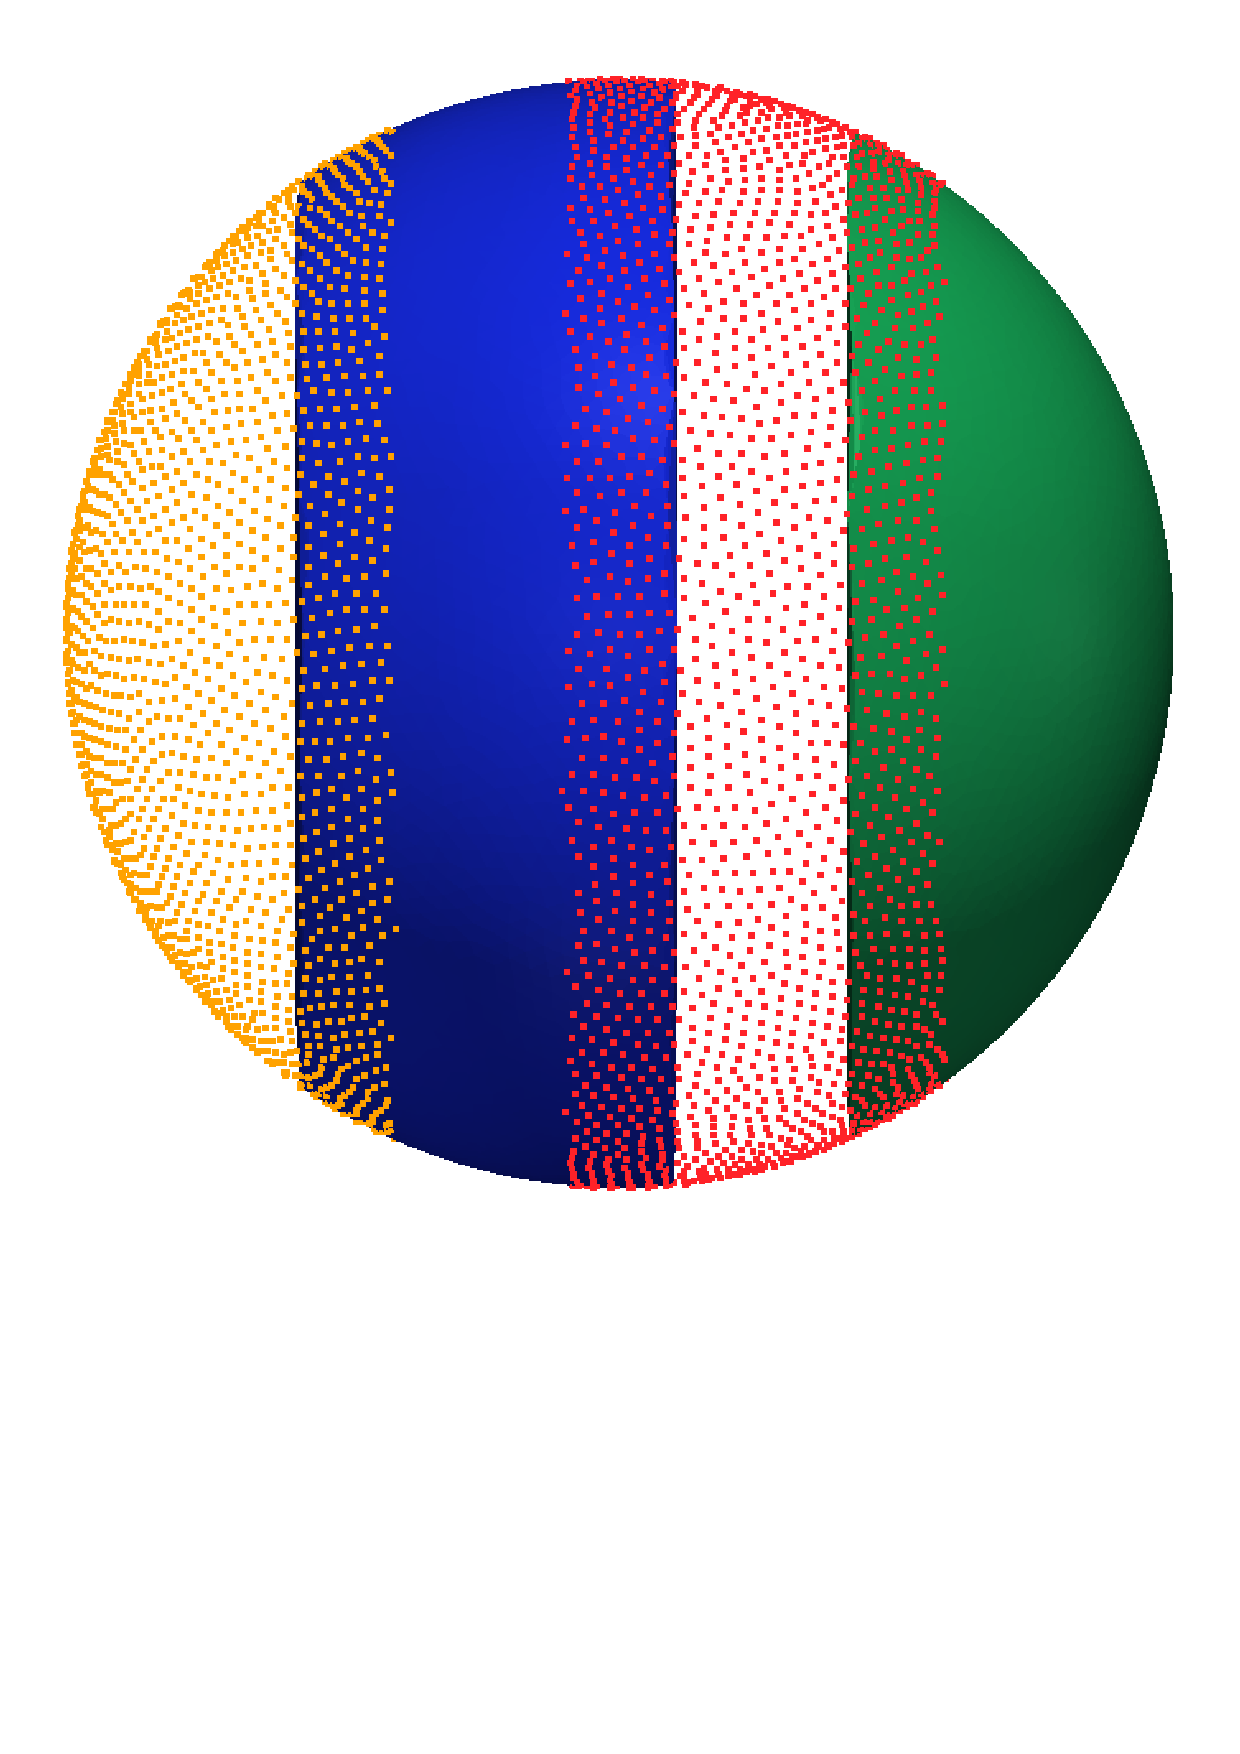
\includegraphics[width=2.5in]{../figures/paper1/figures/vortex_rollup/4procs_N10K_n31.pdf}
\caption{Partitioning of $N=10,201$ nodes to span four processors with stencil size $n=31$. }
\label{fig:decomposed_sphere}
\end{center}
\end{figure}

Linear partitioning is simple and easy to code. Each MPI process has a left and right neighbor, so communication is straightforward. There are two issues with this approach: 
\begin{enumerate} 
\item Scaling the number of processors quickly decreases the width of each partition, and can result in stencils spanning more than one partition in each direction. This introduces the need for complex communication collectives. 
\item In the case of the sphere, the partitioning of near uniform node distributions results in subdomains that are unequal in size and processors are improperly balanced. 
\end{enumerate}

Many other options for partitioning the sphere exist. In atmospheric and geophysical communities for example, one often finds the cubed-sphere \cite{Ivan2011, Katta2012}, which transcribes a subdivided cube onto the sphere and assigns projected rectangular elements to individual processors. Another option is the icosahedral geodesic grid \cite{Randall2002}, which evenly balances the computational load by distributing equal sized geodesic triangles across processors. The options for partitioning the sphere are endless, and are outside the scope of this work. 

%TODO: concept of a domain and subdomains with nodes determined by isInside()

Other interesting partitionings can be generated with software libraries such as the METIS \cite{Karypis1999} family of algorithms, capable of partitioning and reordering directed graphs produced by RBF-FD stencils. 


%TODO: what is the percentage overlap for $n$? $\frac{1}{2} n^{\frac{1}{d}}$ gives depth into neighbor since n is uniformly sampled we expect a cube shape. (SHould be literature on this...no?)} % assume sphere, sqrt of N for scaling area covered by stencil


In order to partition our nodes, METIS requires an undirected adjacency graph representing the edges that connect nodes. In this case the adjacency graph for RBF-FD is directed. The undirected version is constructed with. 

The undirected graph is used only for partitioning and subsequently discarded. 

METIS divides stencils into contiguous partitions of nearly equivalent size. 
%TODO: Need to flesh detail on METIS
%TODO: give overview of how boost graph library is used to construct a sparse adjacency graph

In Figure~\ref{fig:undirected_graph} new non-zeros are introduced to induce symmetry. Since the goal is to partition the physical domain, this added connectivity is harmless to RBF-FD. However, with respect to load balancing, this may not be ideal. For every new nonzero introduced to a row, METIS assumes an additional node utilized by the partition. When the node is a false connection, it is one fewer centers that METIS will assign to the partition in an attempt to keep all partitions balanced. 

%TODO: \authnote{show example of 4 or 8 partitions in table to see how Q, O, R can be disproportionate.}



\begin{figure}[ht!]
\begin{center}
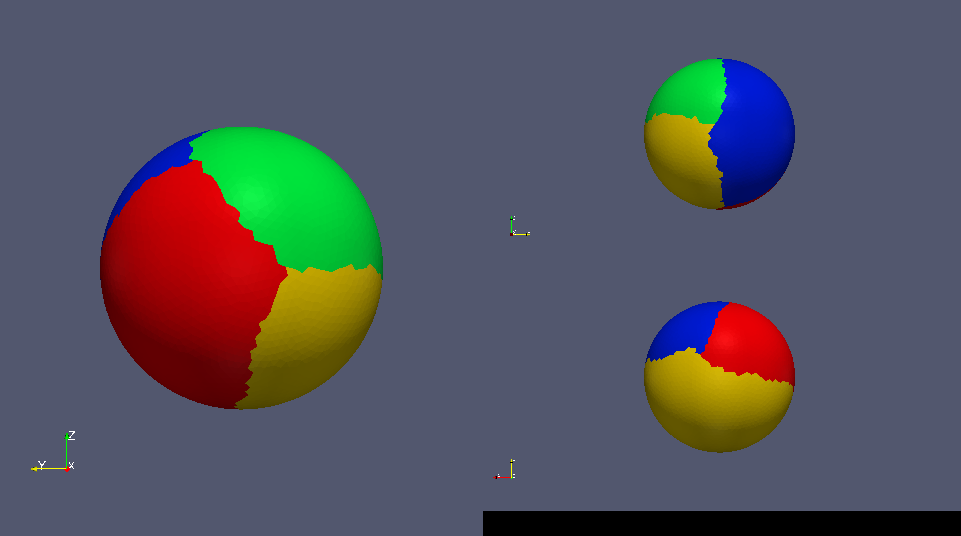
\includegraphics[width=0.8\textwidth]{rbffd_methods_content/decompositions/gpmetis_decomp_sphere_4parts.png}
\caption{METIS partitioning of $N=10,201$ nodes to span four processors with stencil size $n=31$. }
\label{fig:metis_decomposed_sphere}
\end{center}
\end{figure}

%TODO: related work that uses linear partitioning
%Thibault et al. \cite{Thibault200*} use a linear partitioning in the $z$-direction of a 3D cube domain.  
%TODO: related work that uses METIS.




\section{Index Mappings and Local Node Ordering}


\begin{figure}
\begin{center}
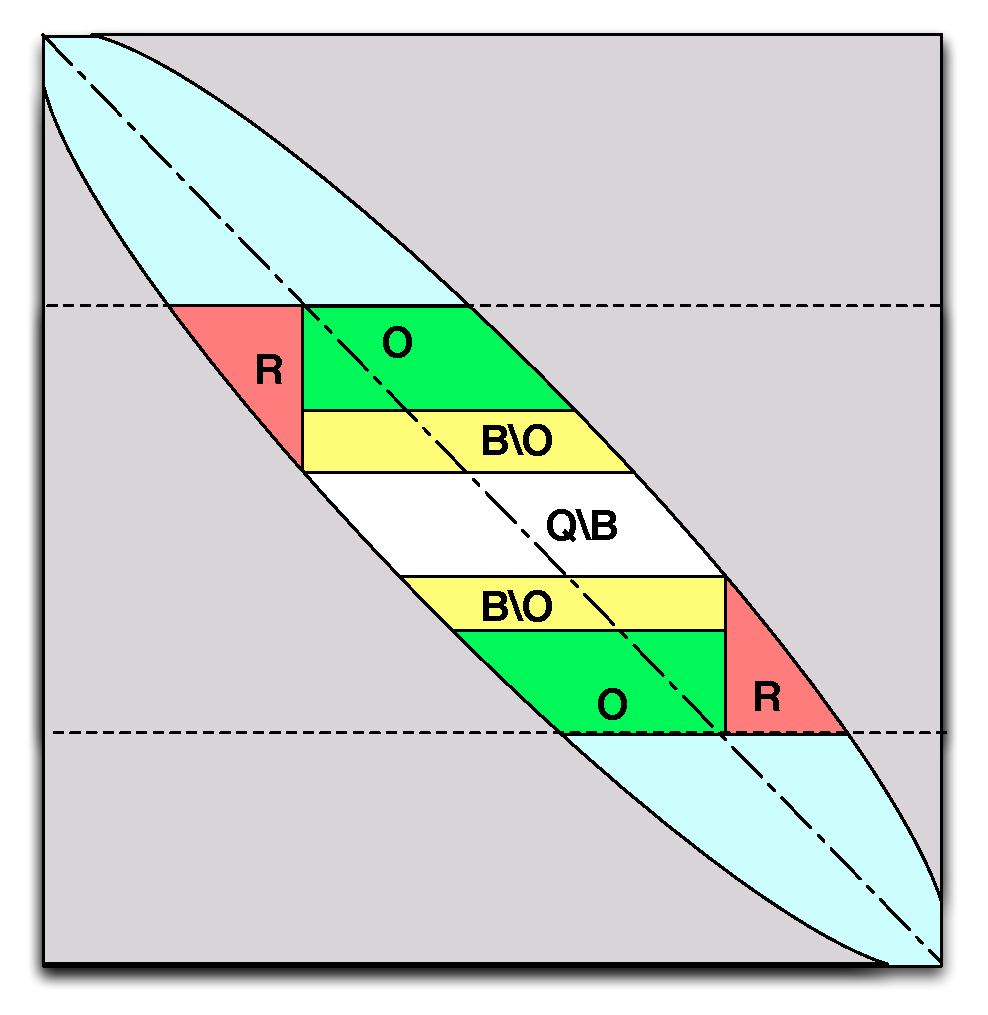
\includegraphics[width=0.45\textwidth]{rbffd_methods_content/decompositions/MatrixDecompositionSets_RBF-FD_Bowed.pdf} 
\caption{Decomposition for one processor selects a subset of rows from the DM. Blocks corresponding to node sets $\setCenters \backslash \setBoundary$, $\setProvide$, and $\setDepend$ are labeled for clarity. The subdomain for the processor is outlined by dashed lines.}
\label{fig:decomp_matrix_view}
\end{center}
\end{figure}



\section{Local node ordering}

After partitioning, each CPU/GPU is responsible for its own subset of nodes. 
To simplify accounting, we track nodes in two ways. Each node is assigned
a global index, that uniquely identifies it. This index follows the node 
and its associated data as it is shuffled between processors. In addition, 
it is important to treat the nodes on each CPU/GPU in an identical manner. 
Implementations on the GPU are more efficient when node indices
are sequential. Therefore, we also assign a local index for the nodes on 
a given CPU, which run from 1 to the maximum number of nodes on that CPU. 

It is convenient to break up the nodes on a given CPU into various sets
according to whether they are sent to other processors, are retrieved from 
other processors, are permanently on the processor, etc. Note as well, 
that each node has a home processor since the RBF nodes are partitioned into 
multiple domains without overlap.
Table~\ref{tbl:stencil_sets}, defines the collection of index lists that each CPU must maintain for both multi-CPU and multi-GPU implementations.  


\begin{figure}[ht!]
\begin{center}
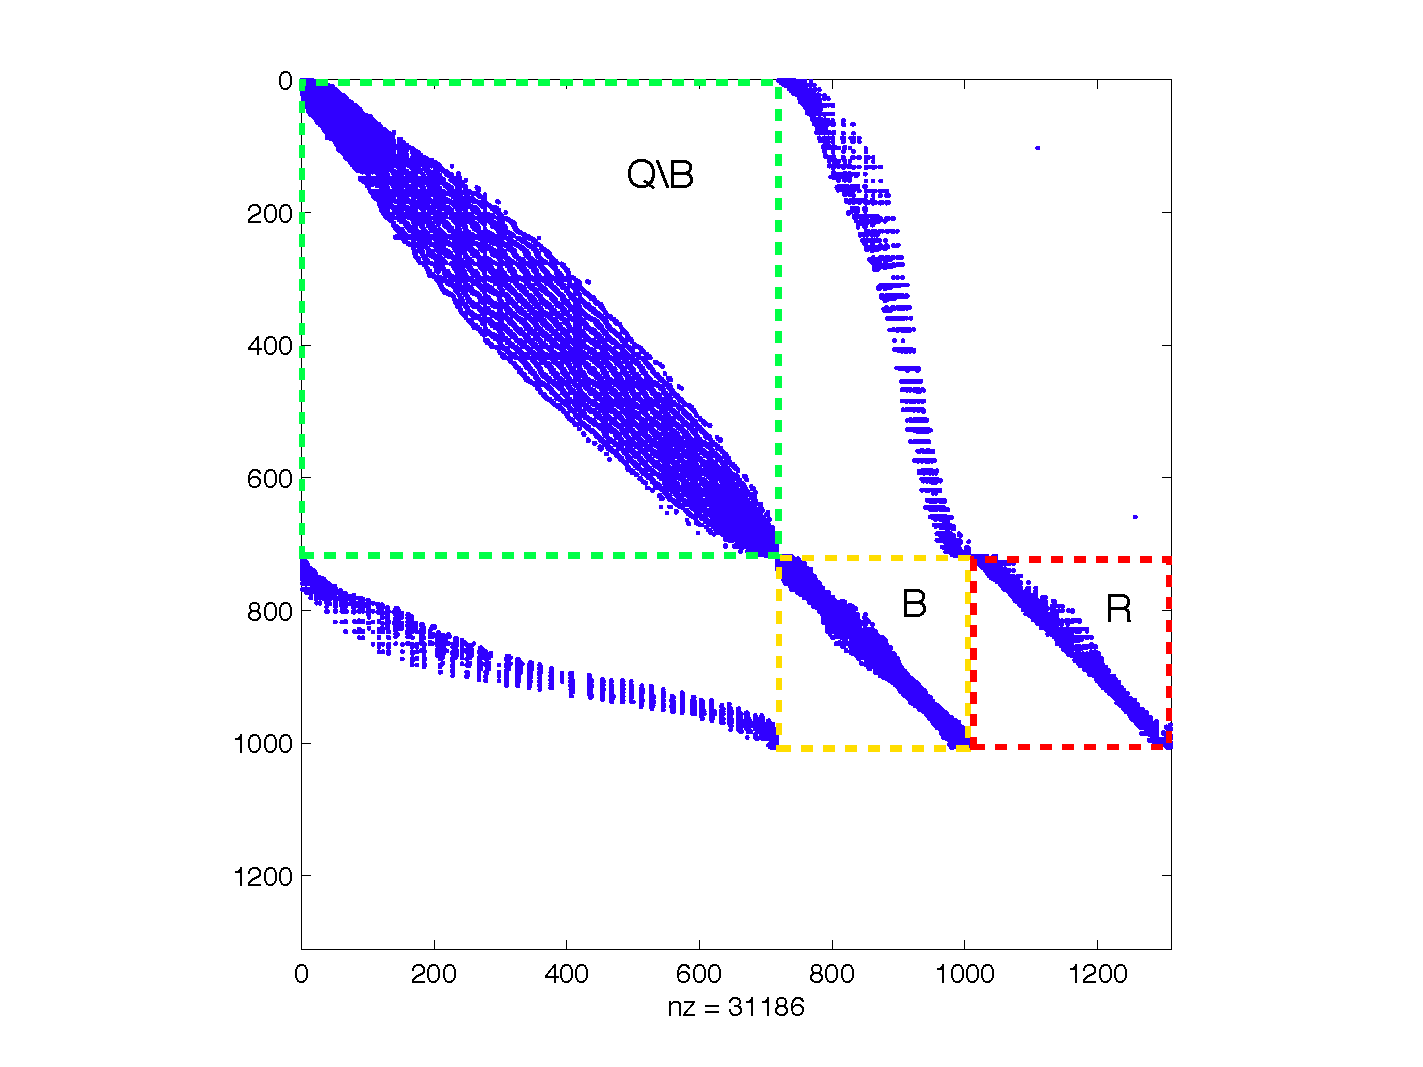
\includegraphics[width=9cm]{rbffd_methods_content/decompositions/spy_metis_stencil_example_labels.png}
%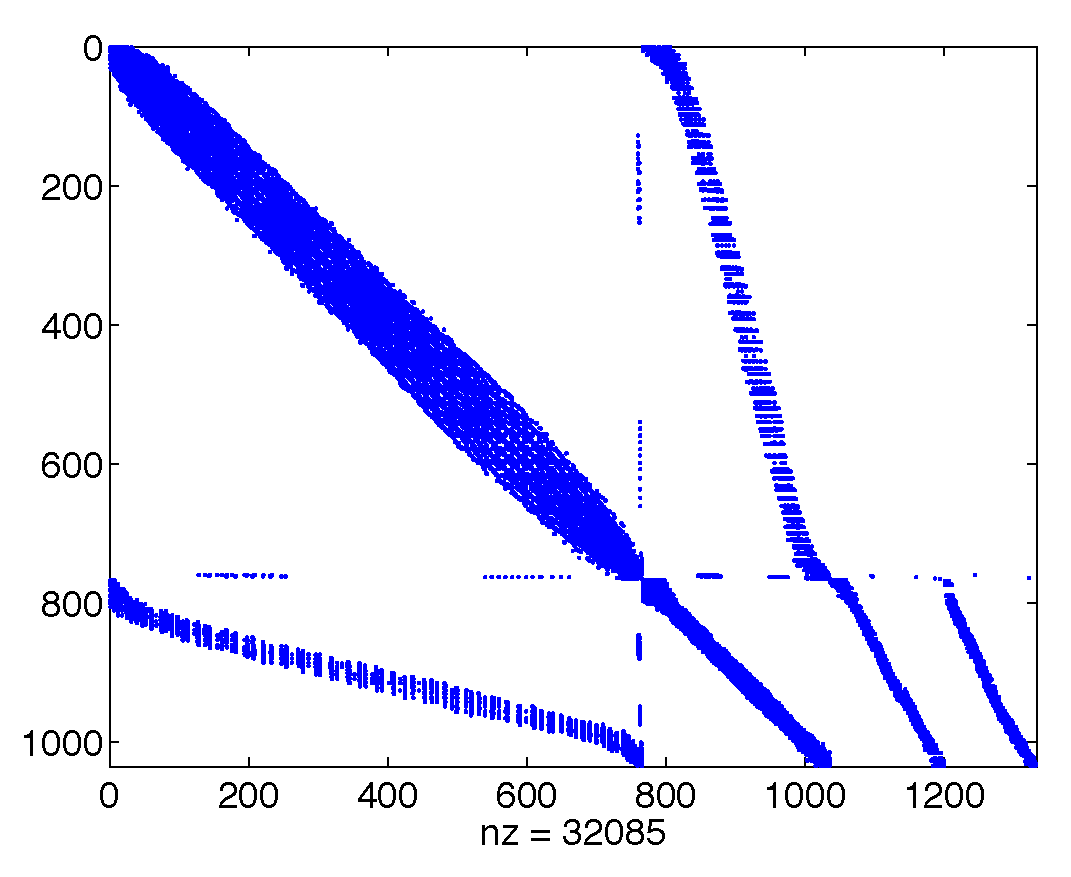
\includegraphics[width=0.45\textwidth]{rbffd_methods_content/decompositions/spy_metis_stencil_example_part_2_of_4.pdf}
\caption{Spy of the sub-DM view on processor 3 of 4 from a METIS partitioning of $N=4096$ nodes with stencil size $n=31$ and stencils generated with Algorithm~\ref{alg:hash_stencils} ($hnx=100$). Blocks are highlighted to distinguish node sets $\setCenters \backslash \setBoundary$, $\setBoundary$, and $\setDepend$. $\setDepend$ Stencils involved in MPI communications have been permuted to the bottom of the matrix. The split in $\setDepend$ indicates communication with two neighboring partitions. }
\label{fig:decomp_spy}
\end{center}
\end{figure}


Figure~\ref{fig:stencilSets2CPU} illustrates a configuration with two 
CPUs and two GPUs, and 9 stencils, four on CPU1, and five on CPU2, separated
by a vertical line in the figure. Each stencil
has size $n=5$. In the top part of the figures, the stencils are laid out
with blue arrows pointing to stencil neighbors and creating the edges of a directed adjacency graph. Note that the connection between two nodes is not 
always bidirectional. For example, node 6 is in the stencil of node 3, but 
node 3 {\em is not\/} a member of the stencil of node 6. 
Gray arrows point to stencil neighbors outside the small window and are not relevant to the following discussion, which focuses only on data flow between 
CPU1 and CPU2. 
Since each CPU is responsible for the derivative evaluation and solution updates for any stencil center, it is clear that some nodes have a stencil with nodes that are on a different CPU. For example, node 8 on CPU1 has a stencil comprised of
nodes 4,5,6,9, and itself. The data associated with node 6 must be retrieved
from CPU2. Similarly, the data from node 5 must be sent to CPU2 to 
complete calculations at the center of node 6.


The set of all nodes that a CPU interacts with is denoted by $\setAllNodes$, which includes not only the nodes stored on the CPU, but the nodes required from other CPUs to complete the calculations. 
The set $\setCenters\in\setAllNodes$ contains the nodes at which the CPU 
will compute derivatives and apply solution updates. 
The set $\setDepend = \setAllNodes \backslash \setCenters$ 
is formed from the set of nodes whose values must be retrieved from another CPU. 
For each CPU, the set $\setProvide\in\setCenters$ is sent to other CPUs. The set $\setBoundary\in\setCenters$ consists of nodes that depend on  values from $\setDepend$ in order to evaluate derivatives. Note that $\setProvide$ and $\setBoundary$ can overlap, but differ in size, since the directed adjacency graph produced by stencil edges is not necessarily symmetric. The set $\setBoundary \backslash \setProvide$ represents nodes that depend on $\setDepend$ but are not sent to other CPUs, while $\setCenters \backslash \setBoundary$ are nodes that have no dependency on information from other CPUs.
The middle section Figure~\ref{fig:stencilSets2CPU} lists global node indices contained in $\setAllNodes$ for each CPU. Global indices are paired with local indices to indicate the node ordering internal to each CPU. The structure of set $\setAllNodes$,
   \begin{equation}
 		\setAllNodes = \{ \mathcal{Q}\backslash\mathcal{B} \ \ \mathcal{B}\backslash\mathcal{O} \ \ \mathcal{O} \ \ \setDepend \},
            \label{eqn:decompose_g}
        \end{equation}
 is designed to simplify both CPU-CPU and CPU-GPU memory transfers by grouping nodes of similar type. The color of the global and local indices in the figure
 indicate the sets to which they belong. They are as follows: white represents $\setCenters \backslash \setBoundary$, 
 yellow represents $\setBoundary \backslash \setProvide$, green indices 
 represent $\setProvide$, and red represent $\setDepend$.  


        \begin{table}[t]
            \begin{center}
                \begin{tabular}{l l}
                    \hline
                    $\setAllNodes$ &: all nodes received and contained on the CPU/GPU $g$ \\
                    $\setCenters$ &: stencil centers managed by $g$ 
					(equivalently, stencils computed by $g$) \\
                    $\setBoundary$ &: stencil centers managed by $g$ that
                    require nodes from another CPU/GPU \\
                    $\setProvide$ &: nodes managed by $g$ that are sent to other CPUs/GPUs  \\
                    $\setDepend$ &: nodes required by $g$ that are managed by another CPU/GPU \\
                    \hline
                \end{tabular}
                \caption{Sets defined for stencil distribution to multiple CPUs}
                            \label{tbl:stencil_sets}
            \end{center}
        \end{table}

        \begin{figure}[ht] 
            \centering
            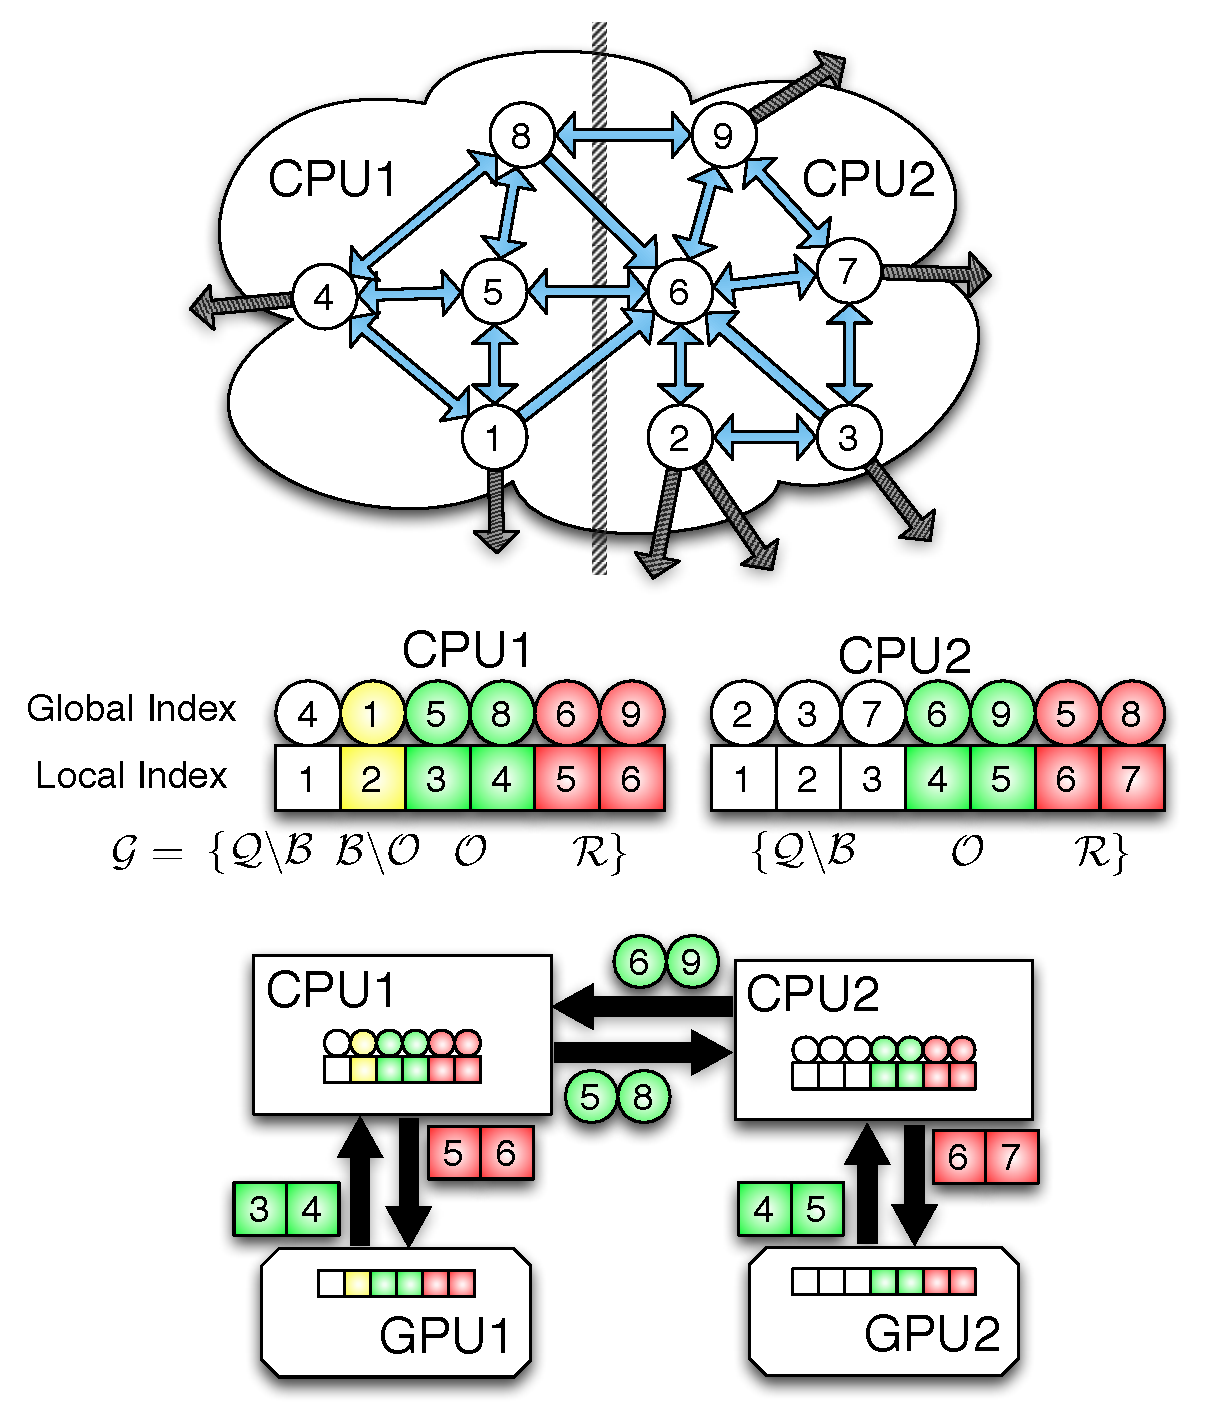
\includegraphics[width=3.5in]{../figures/paper1/figures/omnigraffle/SimpleExample.pdf} 
            \caption{Partitioning, index mappings and memory transfers for nine stencils ($n=5$) spanning two CPUs and two GPUs. Top: the directed graph created by stencil edges is partitioned for two CPUs. Middle: the partitioned stencil centers are reordered locally by each CPU to keep values sent to/received from other CPUs contiguous in memory. Bottom: to synchronize GPUs, CPUs must act as intermediaries for communication and global to local index translation. Middle and Bottom: color coding on indices indicates membership in sets from Table~\ref{tbl:stencil_sets}: $\setCenters \backslash \setBoundary$ is white, $\setBoundary \backslash \setProvide$ is yellow, $\setProvide$ is green and $\setDepend$ is red.
            }
            \label{fig:stencilSets2CPU}
        \end{figure}	

 The structure of $\setAllNodes$ offers two benefits: first, solution values in $\setDepend$ and $\setProvide$ are contiguous in memory and can be copied to or from the GPU without the filtering and/or re-ordering normally required in preparation for efficient data transfers. Second, asynchronous communication allows for the overlap of communication and computation. This will be considered as part of future research on algorithm optimization.  Distinguishing the set $\mathcal{B} \backslash \mathcal{O}$ allows the computation of $\mathcal{Q}\backslash \mathcal{B}$ while waiting on $\mathcal{R}$. 


%TODO: Domain boundary nodes appear at beginning of the list 

Returning to Figure~\ref{fig:decomposed_sphere}, each partition, illustrated
as a unique color, represents set $\setAllNodes$ for a single CPU.  Alternating
representations between node points and interpolated surfaces illustrates the
overlap regions where nodes in sets $\mathcal{O}$ and $\mathcal{R}$ (i.e., nodes
requiring MPI communication) reside. As stencil size increases, the width of the
overlap regions relative to total number of nodes on the sphere also increases. 




When targeting the GPU, communication of solution or intermediate values is a four step process:
        \begin{enumerate}
    \item Transfer $\mathcal{O}$ from GPU to CPU
	\item Distribute $\mathcal{O}$ to other CPUs, receive $R$ from other CPUs
	\item Transfer $\mathcal{R}$ to the GPU
	\item Launch a GPU kernel to operate on $\mathcal{Q}$
     \end{enumerate} 
The data transfers involved in this process are illustrated at the bottom of Figure~\ref{fig:stencilSets2CPU}.
    Each GPU operates on the local indices ordered 
according to Equation~(\ref{eqn:decompose_g}). The set 
$\setProvide$ is copied off the GPU and into CPU memory as one contiguous memory block. The CPU then maps local to global indices and transfers $\setProvide$ to other CPUs. CPUs send only the subset of node values from $\setProvide$ that is required by the destination processors, but it is important to note that node information might be sent to several destinations. 
As the set $\setDepend$ is received, the CPU converts back from global to local indices before copying a contiguous block of memory to the GPU. 


%TODO: \authnote{remember distributed case: no decode}

        This approach is scalable to a very large number of 
		processors, since the individual processors do not require the 
		full mapping between RBF nodes and CPUs. Here scalable is used loosely as there are two types of scaling: weak and strong. Weak scaling implies the total problem size and processor count can increase. The performance scalability of the code depends on the problem size and the MPI collective. In Figure~\ref{fig:strong_scaling} the strong scaling of $N=10^6$ nodes is tested on Itasca, a supercomputer at the Minnesota Supercomputing Institute.   


\section{MPI and Communication Collectives}
\label{sec:mpi_collectives}

It is assumed that the \emph{Message Passing Interface (MPI)} \cite{MPI1993} is used to distribute RBF-FD across an HPC cluster. 


Parallelizing RBF-FD made possible with the Message Passing Interface (MPI). 
MPI history as a standard
MPI supports distributed and shared. 
MPI utilizes the fastest fabric possible for communication, so processes on different cores of the same chip will use shared memory for fastest transfer whereas processes on different nodes might use sockets in the worst case; in reality processes on independent nodes use the Infiniband QDR. 
MPI concept of processes as ranks. Each rank is an independent process with its own memory space. 

MPI collectives are used to share data between processes. Our code leverages three collectives: MPI\_Alltoall, MPI\_Alltoallv and MPI\_Isend/MPI\_Irecv. 

The collective operation is essentially transposing information as seen in Figure~\ref{fig:mpi_alltoallv_visual}. 

An Alltoall collective shares .... as in Figure~\ref{fig:mpi_alltoall_visual}. A basic Alltoall collective would work in most cases. However, RBF-FD stencils are not required/guaranteed to be symmetric. As a result, we often have non-uniform sharing across partitions, so an Alltoall would require over-padding all send/receive buffers to allow the maximum receive size times the number of processors. 

In order to avoid excessive padding, we choose the Alltoallv collective, which allows processors to share non-uniform number of bytes with one another. Figure~\ref{fig:mpi_alltoallv_visual} illustrates the benefit of Alltoallv in comparison to Alltoall (Figure~\ref{fig:mpi_alltoall_visual}. By allowing variable number of bytes, the total message size is reduced for all processors. The downside to an alltoallv




The data in the Itasca scaling figures considers the case where an MPI\_Alltoallv or MPI\_Isend/MPI\_Irecv is used. By issuing the receives before encoding the send buffers we ensure that no processes wait unnecessarily long for their collectives to start.



MPI\_Alltoall requires that all processors send and receive an equivalent number of bytes to one another. Since the size must be equivalent for all processors, the send and receive buffers are padded to the maximum message size for any one connection between processors. MPI\_Alltoallv reduces the number of bytes sent and received by allowing processors to specify variable message sizes when communicating. For a small number of processors the variable message size will function well. However, MPI\_Alltoallv requires all processes to connect with every other process, even in the event that 0 bytes are to be sent. Based on the grid decomposition, processors compute on contiguous partitions with a small number of neighboring partitions. By replacing the MPI\_Alltoallv with a MPI\_Isend/MPI\_Irecv combination, the number of collective connections are truncated such that processors only connect to and communicate with essential neighbors that need/provide data. 

The actual implementation of MPI\_Alltoall and MPI\_Alltoallv likely use Isend and Irecv internally. 

\begin{figure}[ht!]
\begin{center}
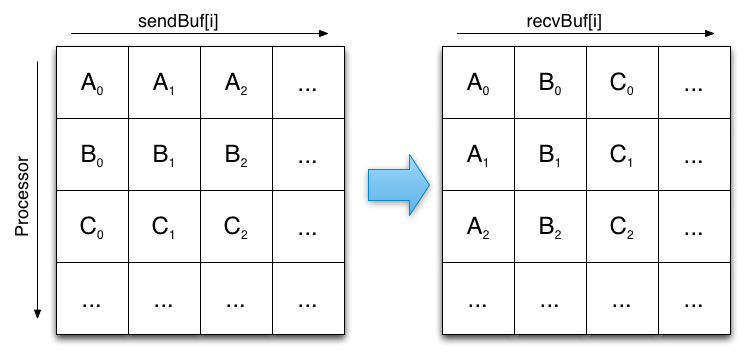
\includegraphics[width=9cm]{../figures/omnigraffle/MPI_Alltoall_Visual.png}
\caption{The MPI\_Alltoall collective allows processors to interchange/transpose data by passing an equivalent number of bytes to every other processor.}
\label{fig:mpi_alltoall_visual}
\end{center}
\end{figure}
\begin{figure}[ht!]
\begin{center}
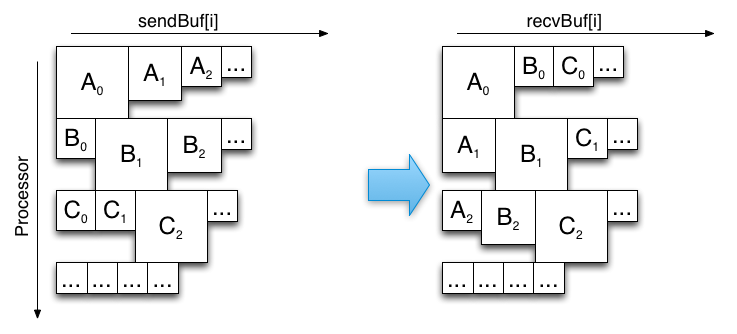
\includegraphics[width=9cm]{../figures/omnigraffle/MPI_Alltoallv_Visual.png}
\caption{The MPI\_Alltoallv collective compresses the interchange from MPI\_Alltoall by allowing for variable message sizes between all processors. Assume message sizes are proportional to square size in figure. When packet sizes are null MPI\_Alltoallv has undefined behavior.}
\label{fig:mpi_alltoallv_visual}
\end{center}

Figure~\ref{fig:mpi_alltoallv_visual}: \url{http://www.mcs.anl.gov/papers/P1699.pdf} observes that the zero-byte messages still add up due to processing required to analyze send-buffer and determine when connection is required. 


\end{figure}
\begin{figure}[ht!]
\begin{center}
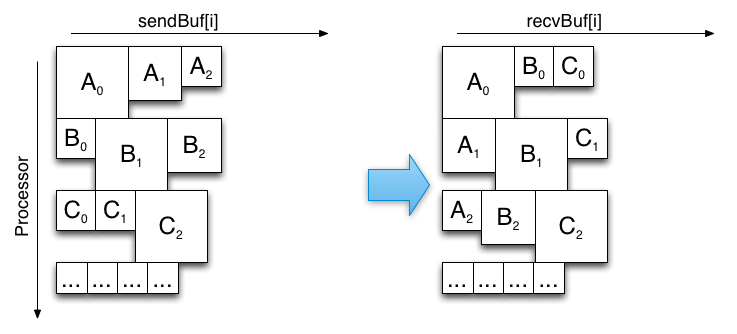
\includegraphics[width=9cm]{../figures/omnigraffle/MPI_IsendIrecv_Visual.png}
\caption{The ``subset-to-subset" (MPI\_Isend/MPI\_Irecv) collective allows for variable message sizes, and truncates the number of connections between processors to only required connections.}
\label{fig:mpi_isendirecv_visual}
\end{center}
\end{figure}

MPI\_Isend/MPI\_Irecv also allows for overlapping communication and computation by posting receives early 

\subsection{Alltoallv}
As a baseline for scaling we start with MPI\_Alltoallv. 

\authnote{figure: alltoall visual} 

\subsection{Isend/Irecv}

The first improvement on Alltoallv collectives is to truncate the number of connections made between processes. Compact stencils implies an overlap region for each processor that draws values from a limited number of neighboring processors. 

\authnote{figure: isend visual}

\subsection{No Decode}
\authnote{figure: per iteration stacked bar for n=50 and 16 processes to show cost of decode}
\authnote{figure: algorithm for collective}

\authnote{figure: alltoall to isend improvement. justify comm\_combo for up to 16 procs.} 
\authnote{figure: comm\_combo gains}
\authnote{figure: algorithm for collective}

\subsection{Immediate Isend on Encode}
\authnote{figure: algorithm for collective}

\authnote{back to section: figure: improvement on all CPU collectives (n=50)}

\authnote{table: show percentage of comm time for actual mpi time. busy network can cause slower comm times. but the decode cost is gone. it can also be an issue if we have saturated comm pipes}



\section{CPU Scaling}

To test and demonstrate scaling of our method, we consider an idealized regular grid in three dimensions. 

verification here is only significant to ensure we are applying all weights. 
We apply weights to calculate derivatives of a test function in X, Y, Z, and the Laplacian. 
the grid is regular and 3D.
We test strong scaling on a $N=160^3$ grid, and weak scaling with $N_p=4000$. This way at $p=1024$ processes we have weak scaling testing the full $N=160^3$ grid. 


\authnote{Show the strong and weak scaling here}

To demonstrate the effectiveness of our decomposition and indexing, we perform scaling experiments. 

\subsection{Strong Scaling}
Strong scaling tests the growth in time for a fixed total problem size, and a variable number of processors. 

\subsection{Weak Scaling}
Weak scaling considers the amount of time for a fixed problem size per process and variable number of processors. That is to say, each processor has roughly the same amount of work, so as we scale to a large number of processors, changes in time will be the result of increased communication overhead. 

Although our weak scaling results are promising, they also contain a problem. First, since we are subsampling a $160^3$ regular grid to get the first $N=p*4000$ nodes, many of the tests consider domains that are ``L" shaped and have odd partitions with limited connectivity.

\authnote{Here and strong scaling: table showing the min and max Osize,Rsize}


\subsection{Bandwidth}

To understand the impact of MPI on these benchmarks we calculate the average and aggregate collective bandwidths. The average bandwidth considers the MPI throughput from the perspective of one processor. 

The aggregate bandwidth reveals when processes saturate the interconnects. 

We consider a simple idealized problem where derivatives are computed over a regular grid generated in 3-D. The experiment computes the SpMV one thousand times. At the end of each SpMV the MPI\_Alltoallv collective is used to synchronize the local derivative vectors. After one thousand iterations, each process computes the local norm of the resulting vector and an MPI\_Reduce collective dra


\begin{figure} 
\centering
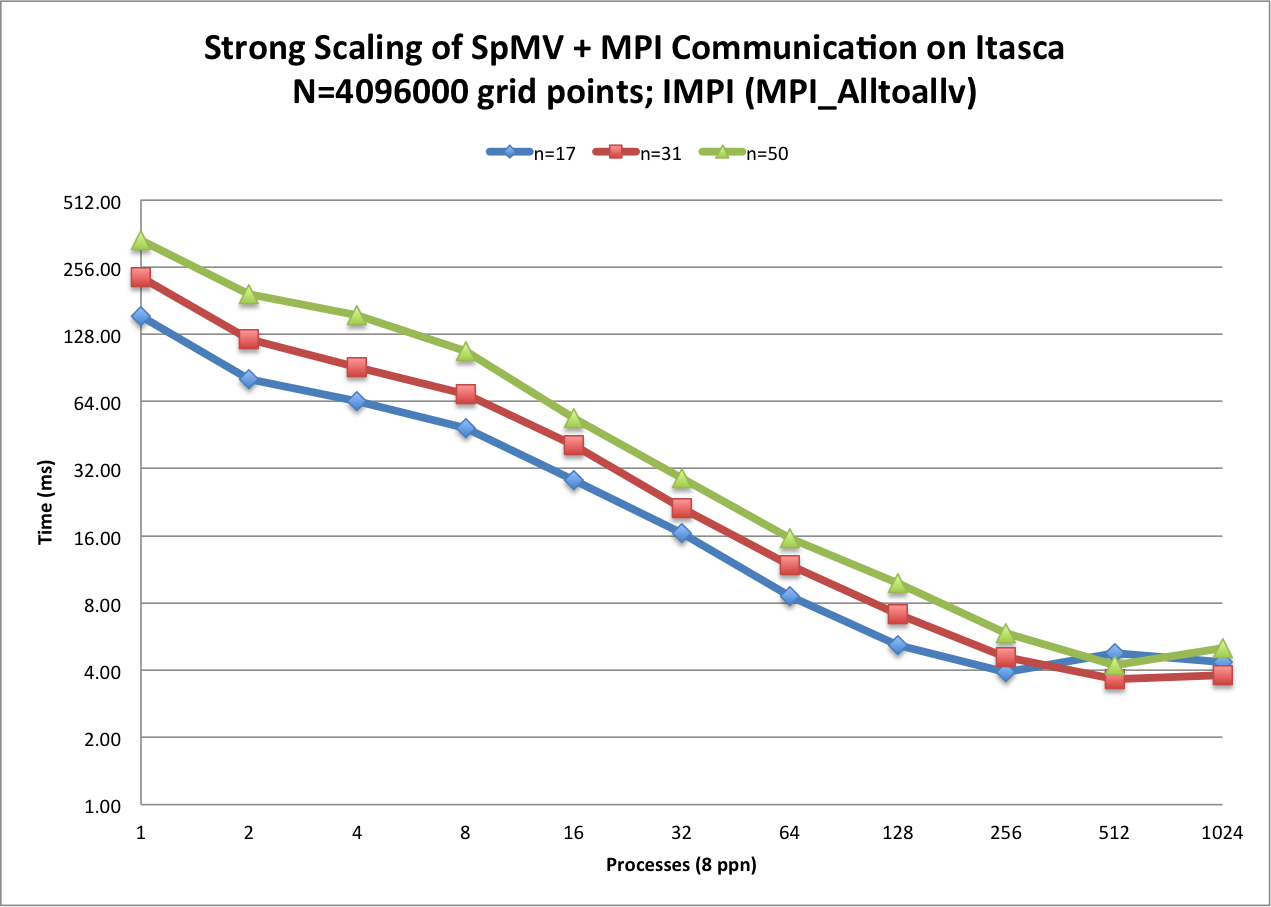
\includegraphics[width=0.45\textwidth]{performance_content/scaling/strong_scaling_4M_regular_alltoallv.png}  
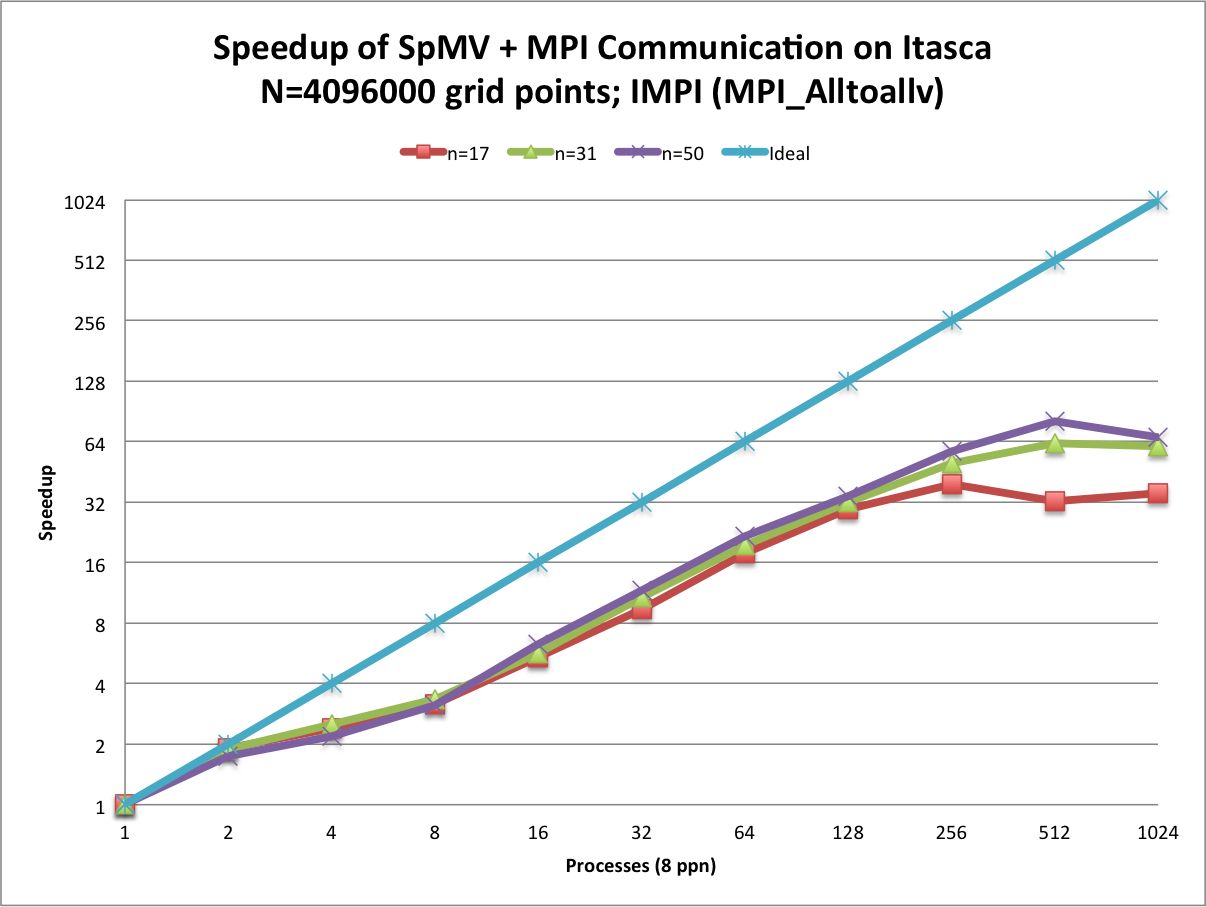
\includegraphics[width=0.45\textwidth]{performance_content/scaling/strong_scaling_4M_regular_alltoallv_speedup.png} \\
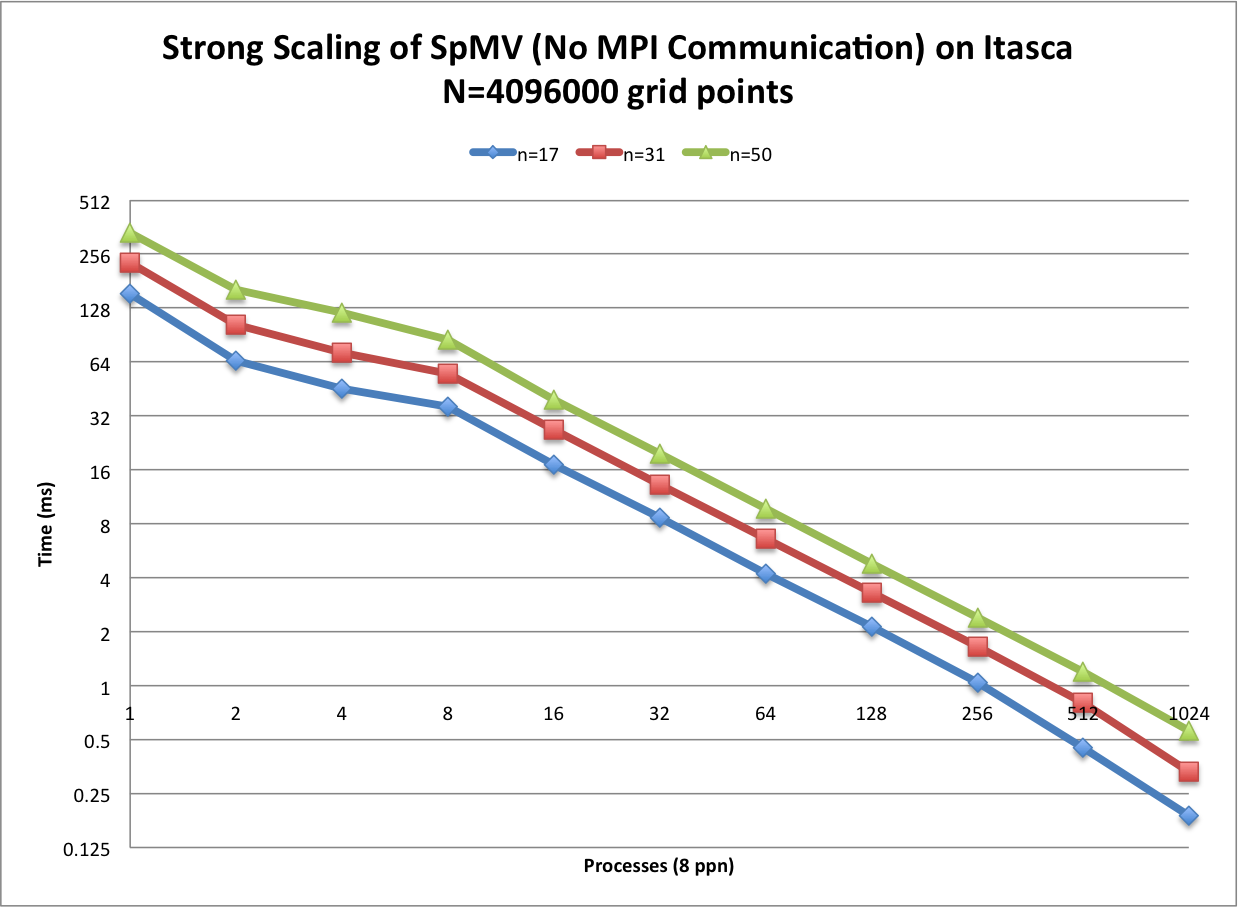
\includegraphics[width=0.45\textwidth]{performance_content/scaling/strong_scaling_4M_regular_spmvOnly.png}
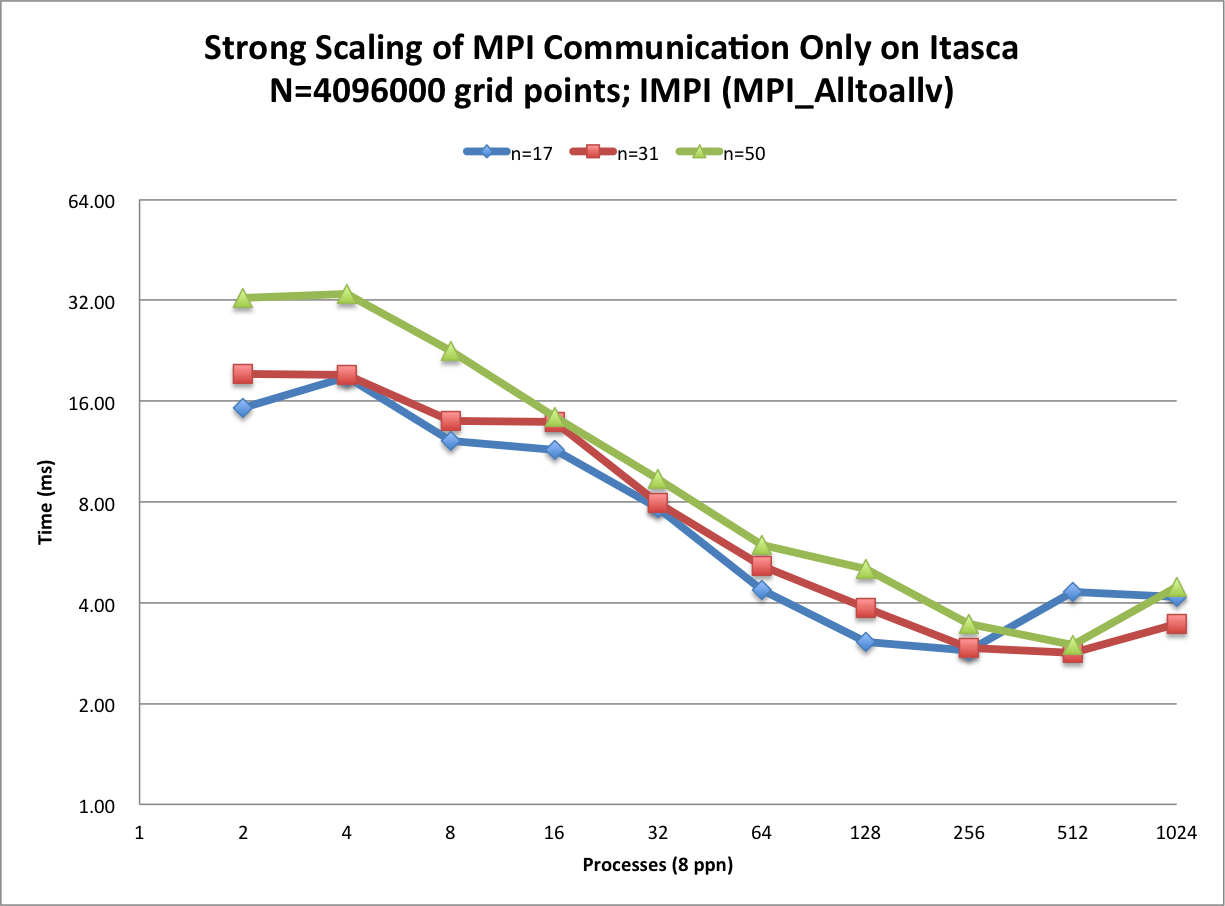
\includegraphics[width=0.45\textwidth]{performance_content/scaling/strong_scaling_4M_regular_alltoallv_commOnly.png} 
\caption{Strong scaling the distributed SpMV for $N=4096000$ nodes (i.e., a $160^3$ regular grid) and various stencil sizes. Here the MPI\_Alltoallv collective operation is used. (Left) Strong scaling of SpMV (including cost of communication). (Center) Strong scaling of computation only. (Right) Strong scaling of communication only.}
\end{figure}

\begin{figure}
\centering
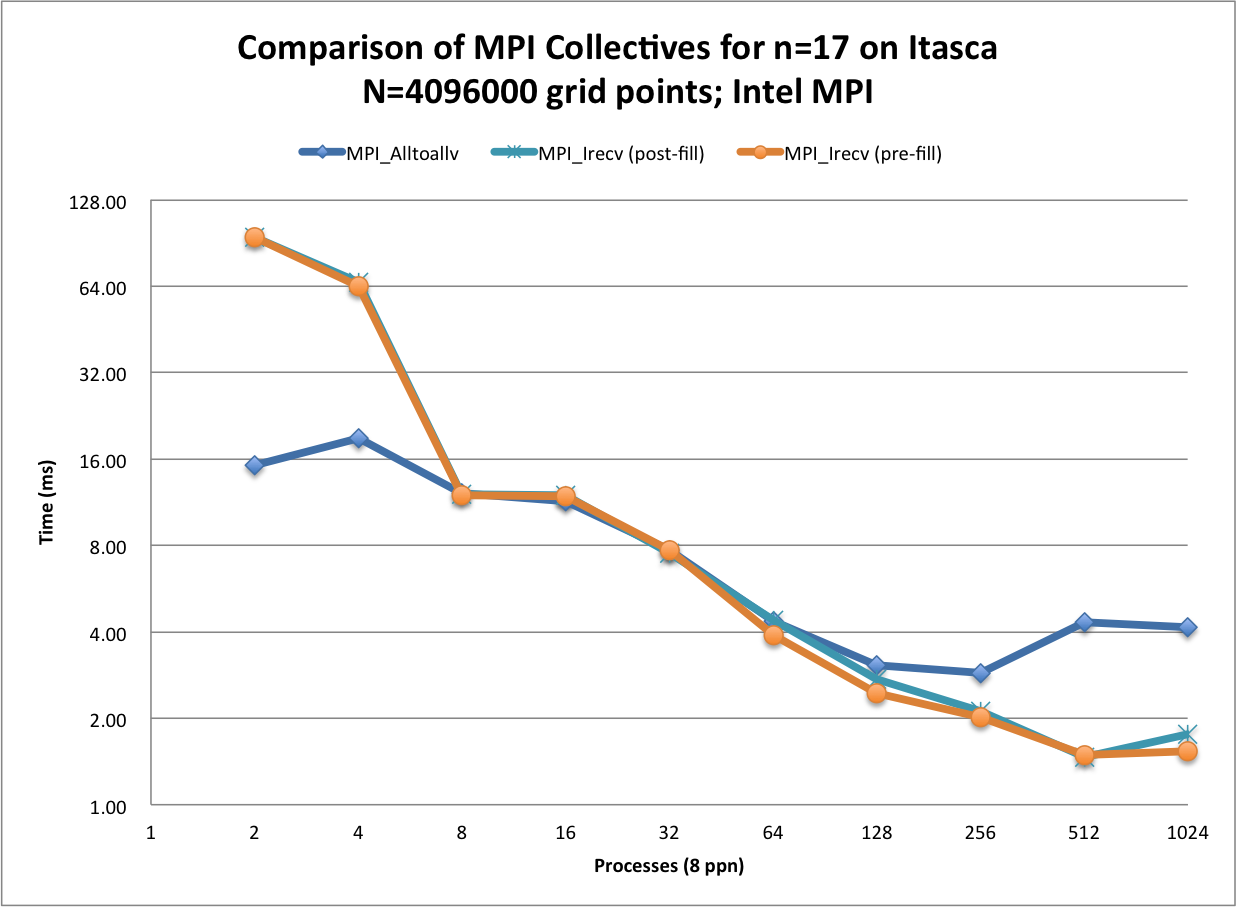
\includegraphics[width=0.6\textwidth]{performance_content/scaling/strong_scaling_4M_regular_n17comparison_commOnly.png}
\caption{Scaling comparison of MPI\_Alltoallv and two types of MPI\_Isend/MPI\_Irecv collectives: one with MPI\_Irecv issued after filling the MPI\_Isend send buffer (post-fill), and the other issued before filling the MPI\_Isend buffer (pre-fill).}
\end{figure}

\begin{figure}
\centering
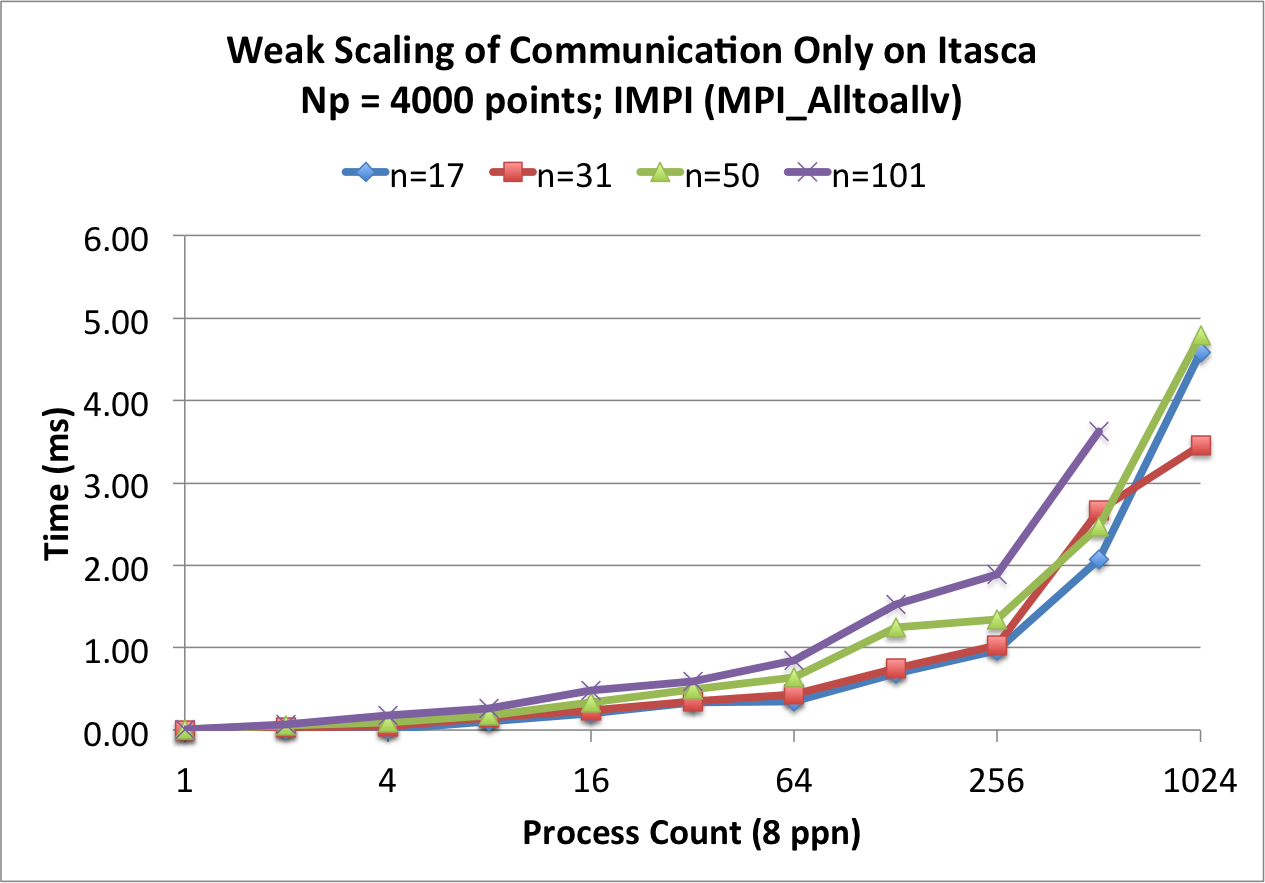
\includegraphics[width=0.45\textwidth]{performance_content/scaling/weak_scaling_np4000_regular_alltoallv_commOnly.png}
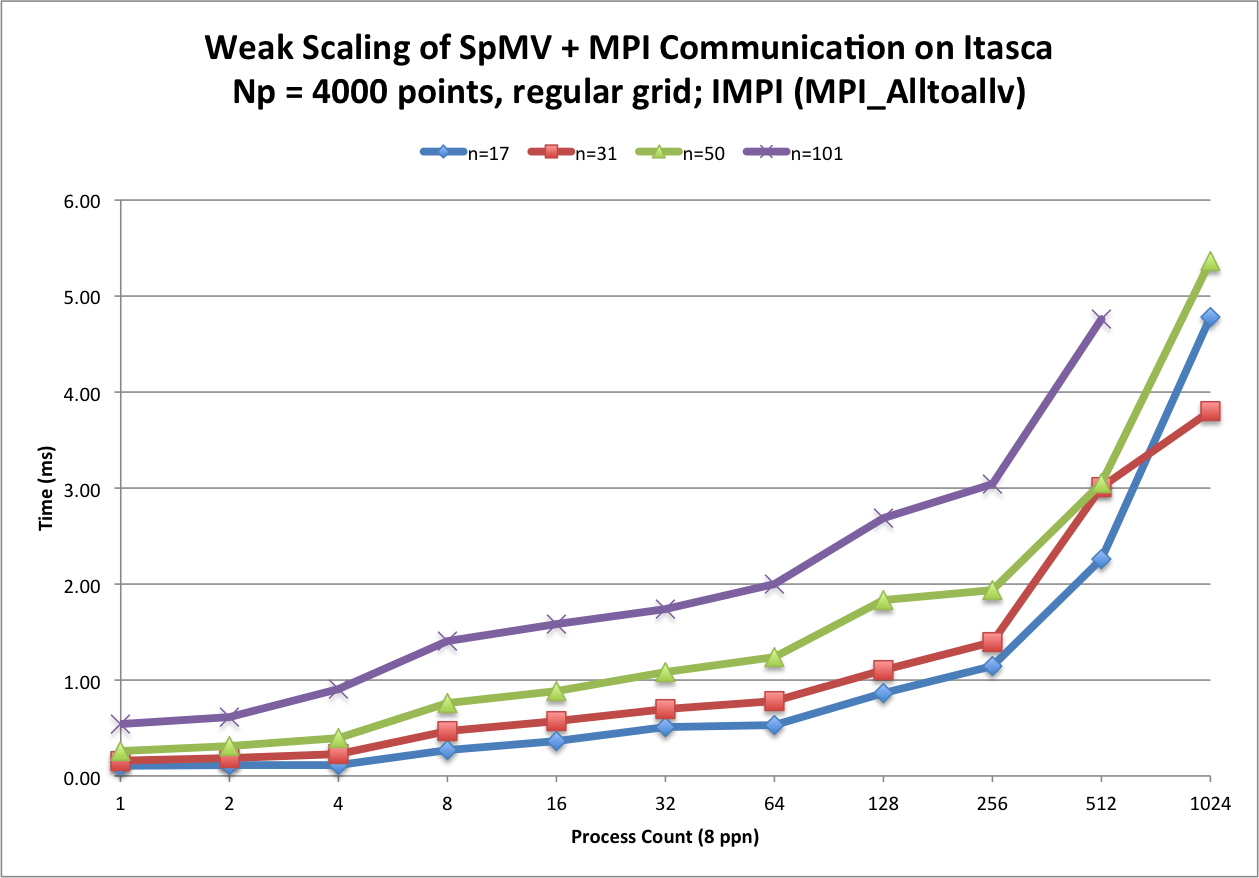
\includegraphics[width=0.45\textwidth]{performance_content/scaling/weak_scaling_np4000_regular_alltoallv.png}  
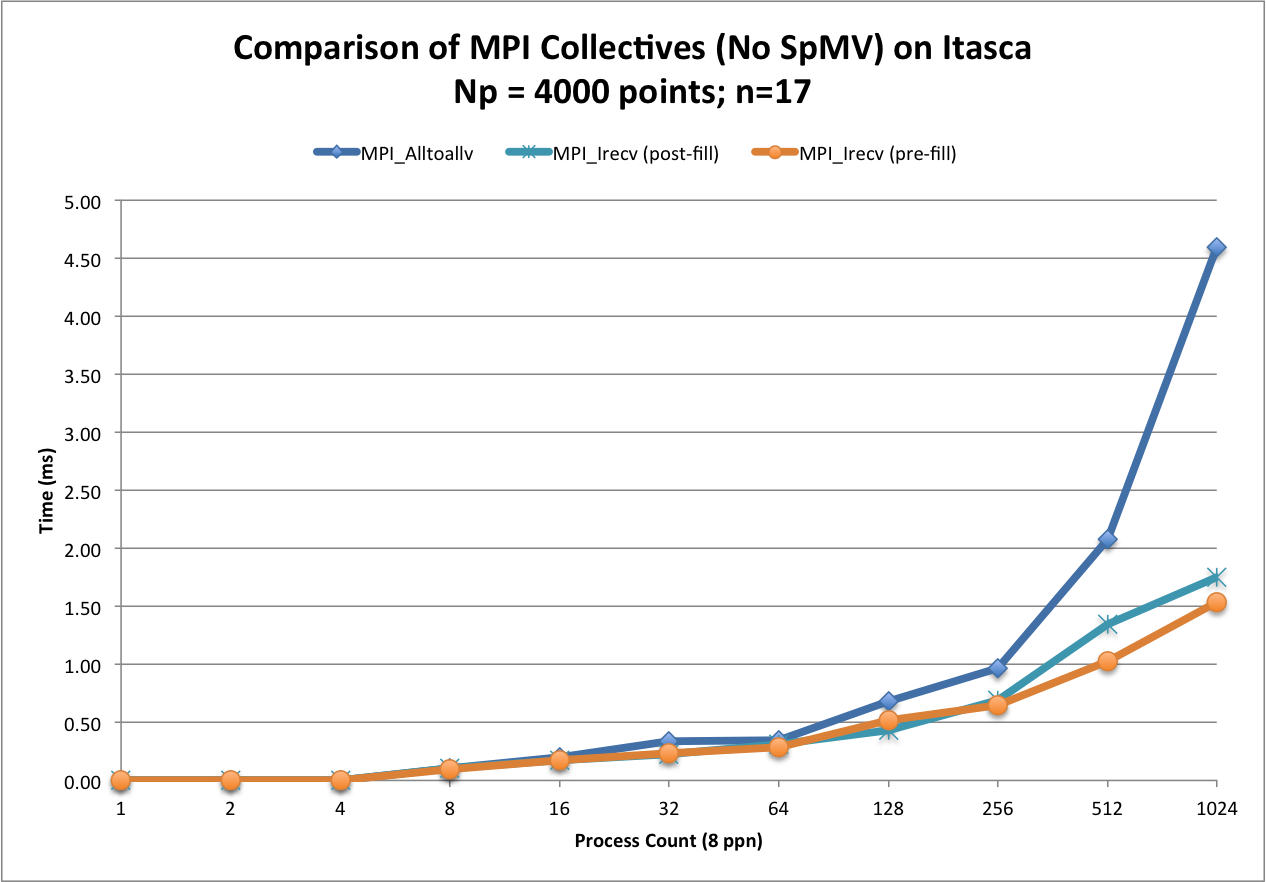
\includegraphics[width=0.45\textwidth]{performance_content/scaling/weak_scaling_np4000_regular_n17_compare_commOnly.png} \\
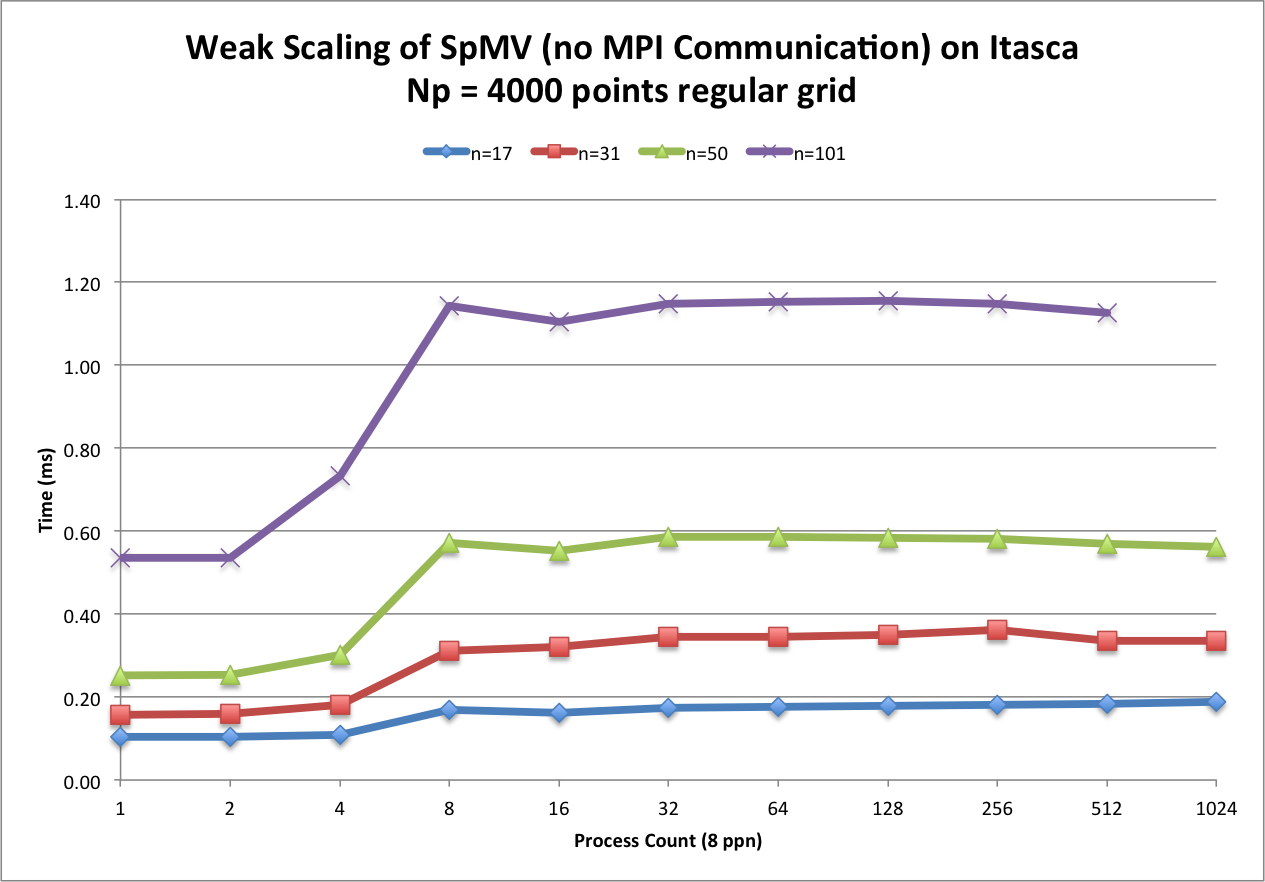
\includegraphics[width=0.45\textwidth]{performance_content/scaling/weak_scaling_np4000_regular_spmvOnly.png} 
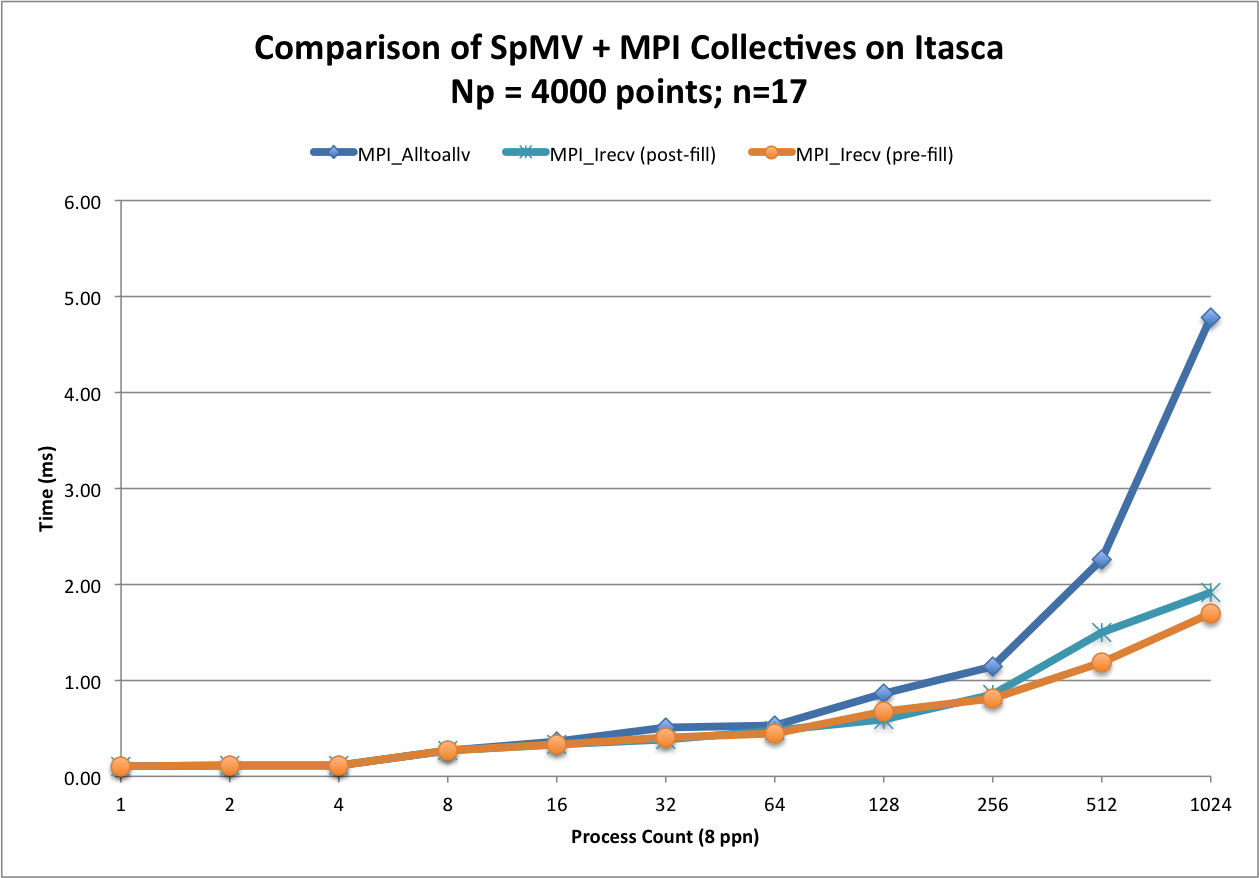
\includegraphics[width=0.45\textwidth]{performance_content/scaling/weak_scaling_np4000_regular_n17_compare.png}
\caption{Weak scaling of the SpMV}
\end{figure}


\begin{figure}
\centering
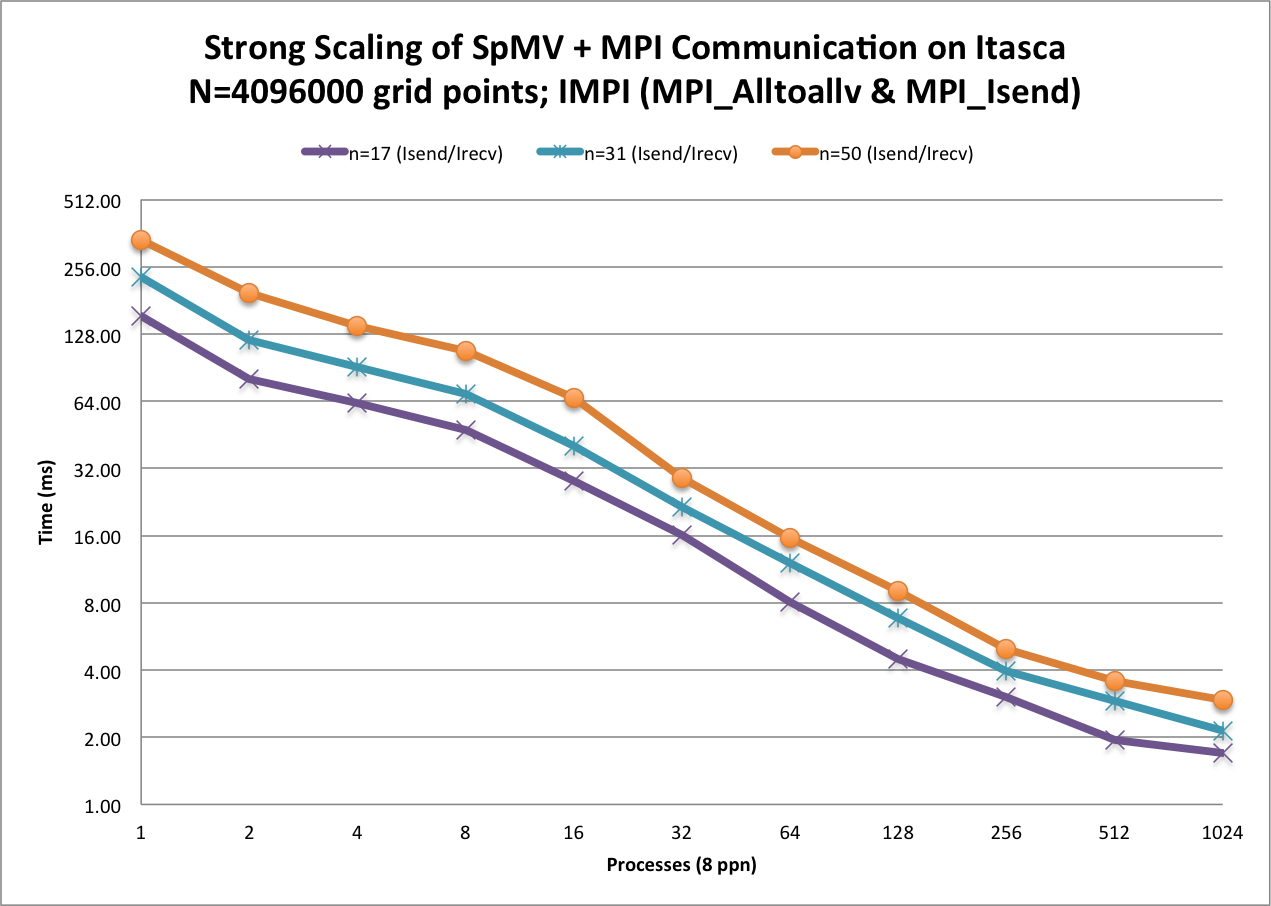
\includegraphics[width=0.45\textwidth]{performance_content/scaling/strong_scaling_4M_regular_isend.png}  
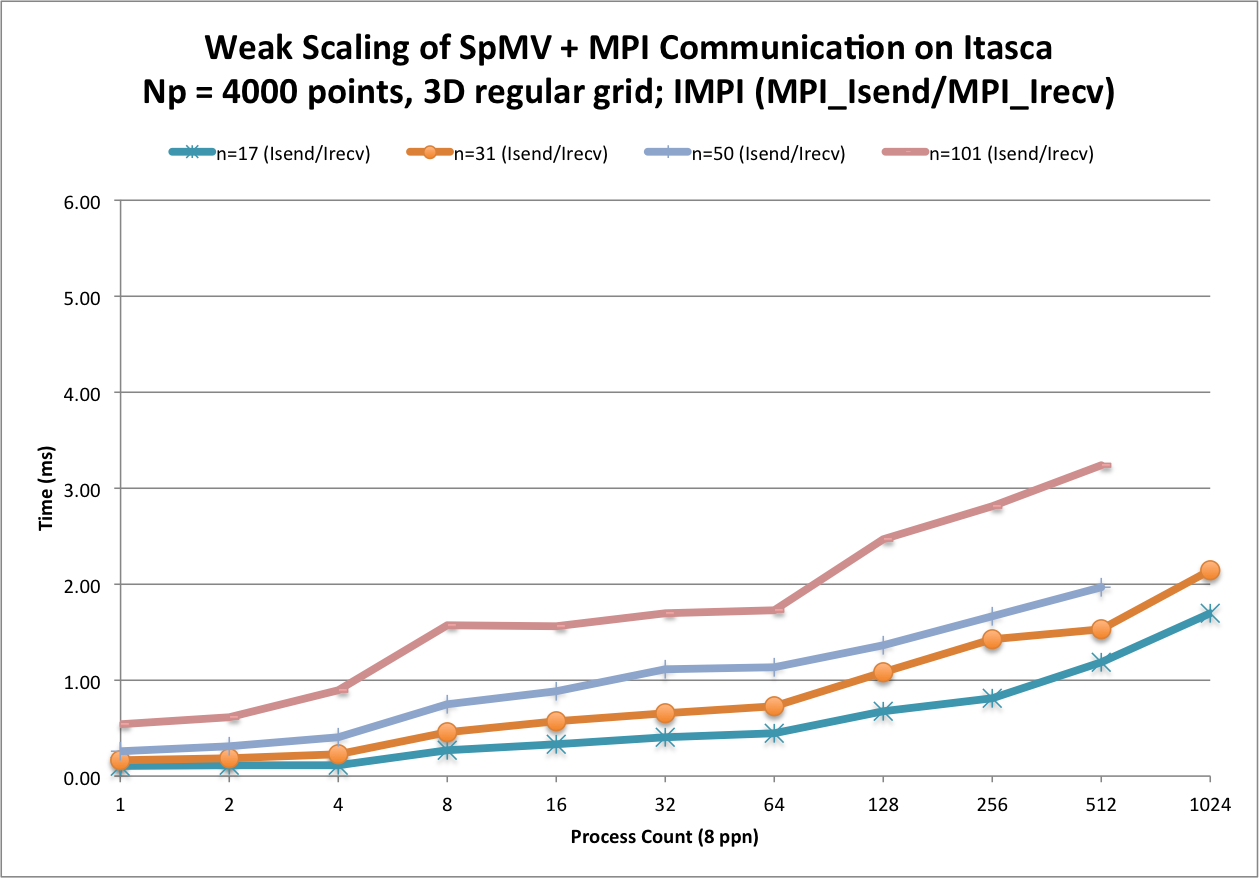
\includegraphics[width=0.45\textwidth]{performance_content/scaling/weak_scaling_np4000_regular_isend.png}  
\caption{Scaling of SpMV with MPI\_Isend/MPI\_Irecv}
\end{figure}


\chapter{Distributed GPU SpMV (incomplete)}
\label{chap:multigpu_rbffd}

Distributing SpMV across multiple GPUs poses a new problem: as previous mentioned, the data sent and received via MPI collectives must be copied from device to host and vice-versa. To amortize this cost we introduce a novel overlapping algorithm to hide the cost of communication behind the cost of a concurrent SpMV on the GPU. 


Petascale computing centers around the world are leveraging GPU accelerators to achieve peak performance. In fact, many of today's high performance computing installations boast significantly more GPU accelerators than CPU counterparts. The Keeneland project is one such example, currently with 240 CPUs accompanied by 360 NVidia Fermi class GPUs with at least double that number expected by the end of 2012 \cite{Vetter2011}. 

Such throughput oriented architectures require developers to decompose problems into thousands of independent parallel tasks in order to fully harness the capabilities of the hardware. To this end, a plethora of research has been dedicated to researching algorithms in all fields of computational science. Of interest to us are methods for atmospheric- and geo-sciences. 

\section{Overlapped Queues}

\section{Avoiding Copy Out}
When operating on multiple GPUs we avoid the copy-out or decode phase by requiring that the local ordering of nodes sort the set $\setDepend$ by the rank of the process sending each node. This way, when the MPI collective finishes and all values arrive contiguous by provider, the data can be copied directly to the GPU without reordering.




\subsection{Avoiding Copy-Out on CPU}

\section{Scaling}
We scale the SpMV across the GPUs on Cascade.

\subsection{Fermi}
\subsection{Kepler}
\subsection{Multiple Kernel Scheduling}
describe fermi's ability to schedule multiple kernels, what it means for our queues. Do we need multiple queues, or just one that is non-blocking. How do we indicate we are done communicating if there is no queue to add markers to? 


\section{HPC Spear Cluster} 

\section{Keeneland}

\subsection{Shared K20s}



\section{Future Work}

One of the problems with choosing to work in OpenCL is the fact that the standard offers the lowest common denominator of features from the various hardware vendors that support it. Many vendor specific features never make it into the language. 

Take for example GPUDirect, a technology introduced first CUDA v3.1 for NVidia hardware. GPUDirect allows direct access to GPU memory addresses from various sources including other GPUs. The technology allows GPUs to bypass copies to host memory en-route to another GPU on the same compute node. Combine GPUDirect with the new MPI aware features in CUDA v5.0 and data can pass directly from a GPU onto the infiniband fabric and up to another GPU \cite{NvidiaGPUMPI}. This type of feature may never be available in OpenCL. 




\ifstandalone
\bibliographystyle{plain}
\bibliography{merged_references}
\end{document}
\else
\expandafter\endinput
\fi

